\documentclass[12pt,a4paper]{article}
\usepackage[utf8]{inputenc}
\usepackage{amsmath}
\usepackage{amsfonts}
\usepackage{amssymb}
\usepackage{graphicx}
\graphicspath{ {./img/} }
\usepackage{hyperref}

\usepackage[a4paper, total={6in, 8in}]{geometry}

\author{Natale Guadagno, Paolo Patrone}
\title{Problem Statement - TecStore}
\renewcommand{\contentsname}{Contenuti}

\usepackage{hyperref}
\hypersetup{
    colorlinks,
	citecolor=blue,
    filecolor=blue,
    linkcolor=blue,
    urlcolor=blue,
    linktocpage
}

\begin{document}

\maketitle
\newpage
\tableofcontents
\newpage

\section*{Partecipanti}
\begin{center}
\begin{tabular} {|c|c|}
\hline
\textbf{Nome} & \textbf{Matricola} \\
\hline
Guadagno Natale & 0512106546 \\
Patrone Paolo & 0512106153 \\
\hline
\end{tabular}
\end{center}


\section*{Revision History}
\begin{center}
\begin{tabular} {|c|c|c|}
\hline
\textbf{Data} & \textbf{Versione} & \textbf{Descrizione} \\
\hline
24/10/2021 & 0.1 & Prima stesura \\
30/11/2021 & 0.2 & Revisione generale \\
\hline
\end{tabular}
\end{center}

\newpage

\section{Dominio del problema}
Il commercio on-line è una delle attività che sono divenute possibili solo con l'avvento di Internet. Nato alla fine degli anni '90, è ormai il punto di forza di aziende che hanno alcuni dei fatturati annuali più alti in assoluto. Prendendo l'anno 2020 come riferimento, aziende come Amazon (386 miliardi di dollari USA\footnote{https://finance.yahoo.com/quote/AMZN/financials?p=AMZN}), il gruppo Alibaba (112 miliardi complessivi in dollari USA\footnote{https://finance.yahoo.com/quote/BABA/financials?p=BABA}), eBay (10 miliardi di dollari USA\footnote{https://finance.yahoo.com/quote/EBAY/financials?p=EBAY}) e altre ancora hanno registrato incassi record.

Ci si propone quindi come obiettivo la realizzazione di una piattaforma di e-commerce altamente specializzato in componentistica tecnologica. \\

\noindent
Il funzionamento previsto non è dissimile da altre piattaforme esistenti, con un \emph{frontend} riservato all'utenza che permette agli utenti non registrati di consultare il catalogo di articoli messi in vendita dalla piattaforma o da altri utenti e, per gli utenti registrati di acquistare articoli, una funzionalità di "carrello" che permetta agli utenti di continuare gli acquisti in un momento successivo e, la possibilità, per utenti che lo desiderano, di mettere in vendita articoli.

A ciò si aggiunge un \emph{backend} con più viste, riservate al personale, che permette la gestione degli ordini per i magazzinieri, la gestione delle richieste dell'utenza (\emph{ticket}) per i centralinisti, la modifica del personale per l'addetto al personale, la gestione del catalogo per l'addetto alla merce.


\newpage
\section{Scenari}
\subsection{Un utente non registrato vuole acquistare un articolo}
\textbf{Attore:} Luca Garibaldi, utente non registrato e Massimo Boni, magazziniere \\
\noindent
\textbf{Flusso di eventi:}
\begin{enumerate}
\item Luca ha deciso di effettuare un upgrade al suo computer.

\item Non convinto dai prezzi dei principali venditori, decide di cercare un negozio alternativo e si imbatte in TecStore.

\item Cercando tra le CPU compatibili con la sua scheda madre, si imbatte nella CPU "Intel i5 10400f" a un prezzo scontato rispetto alla concorrenza e decide quindi di effettuare l'acquisto.

\item Aggiunge il componente al carrello. \\

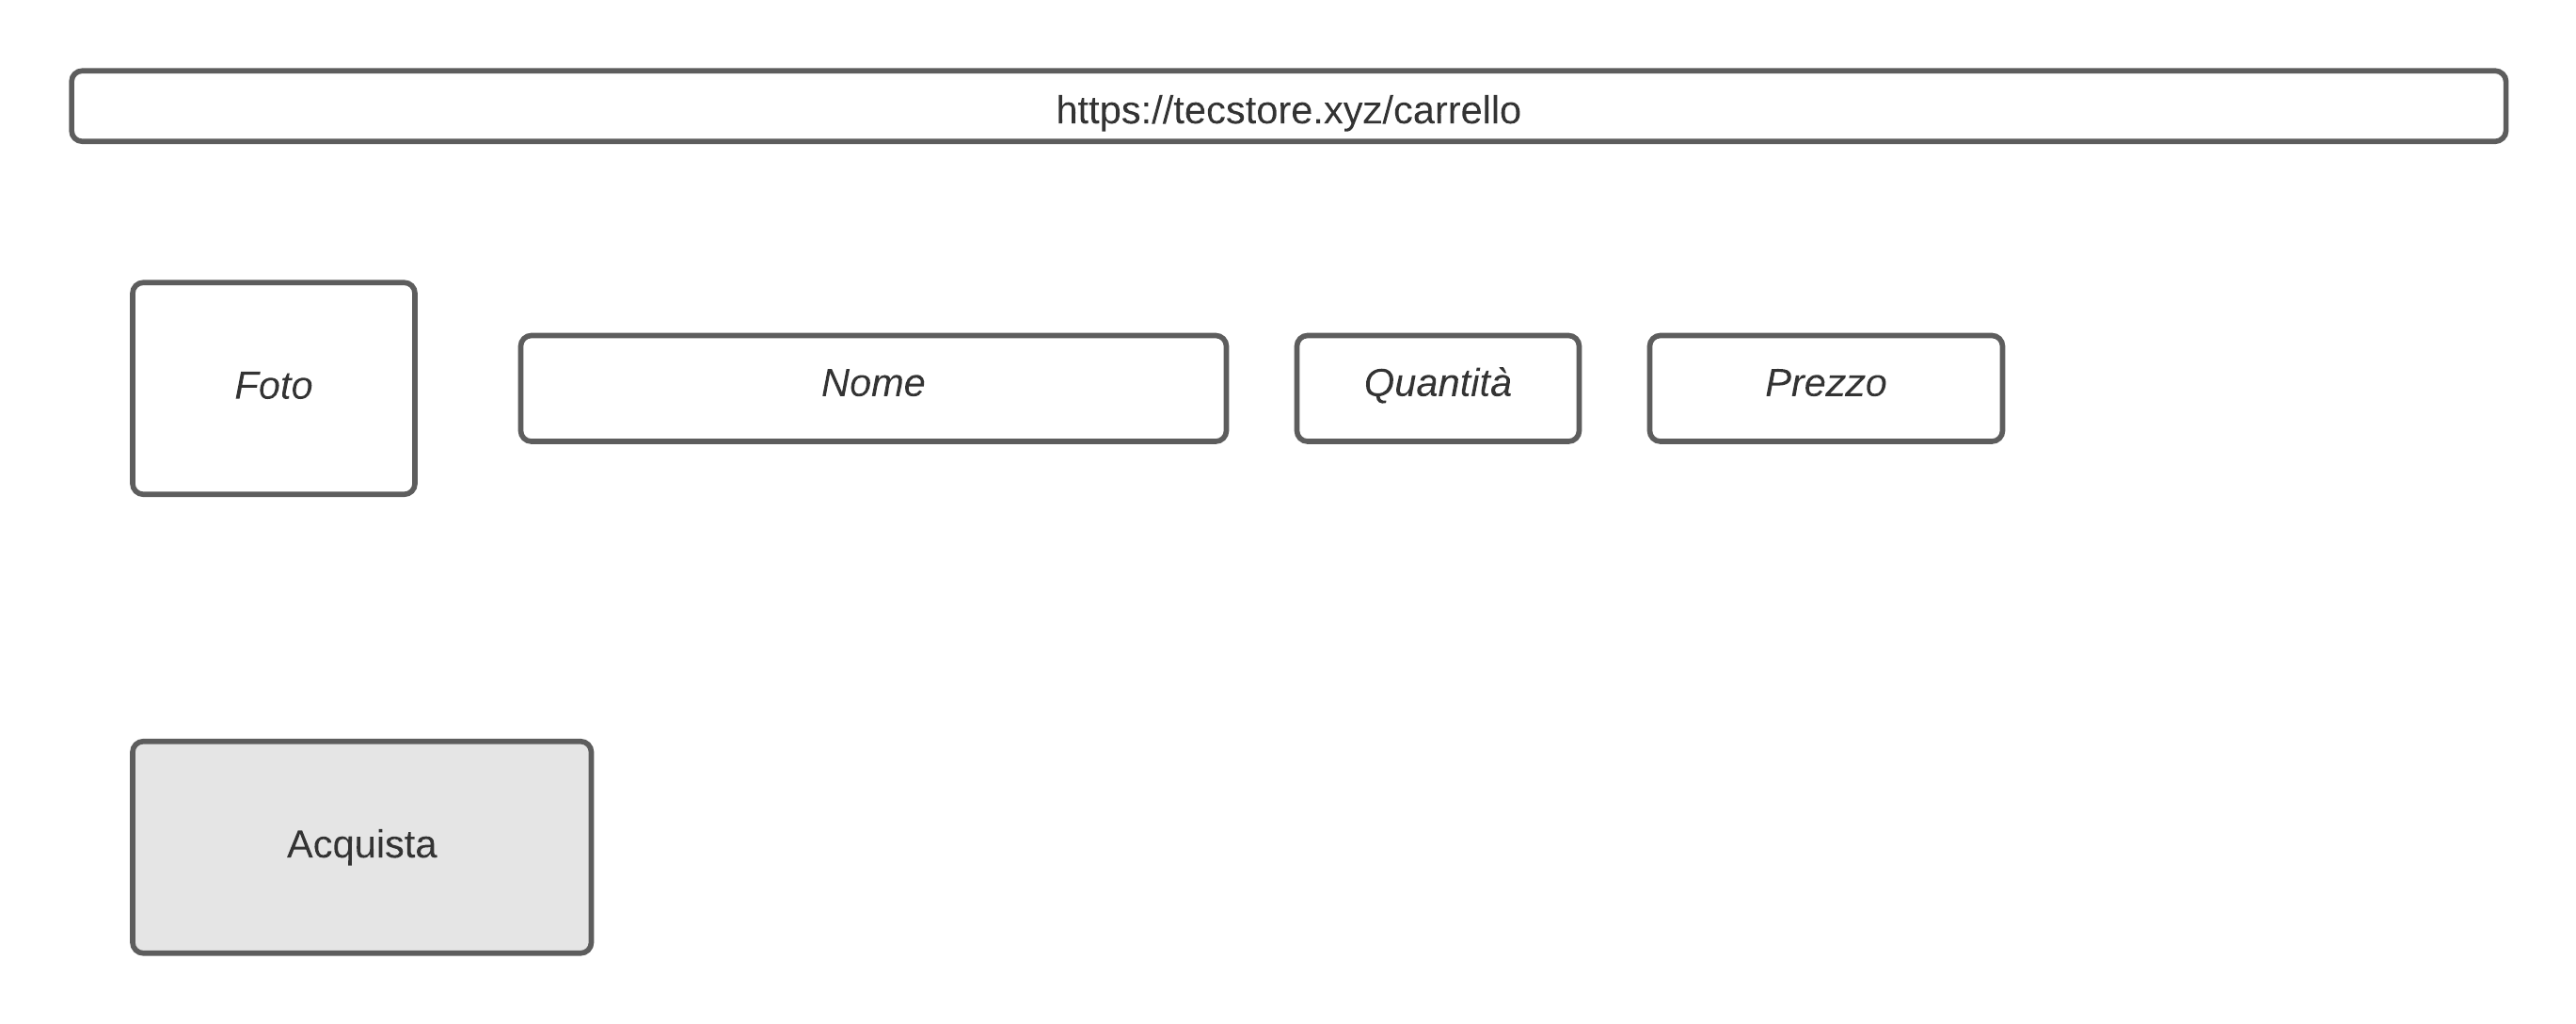
\includegraphics[height=150px]{carrello}

\item Fa click sul tasto per effettuare l'ordine e gli viene chiesto di effettuare il login. Dato che non è ancora utente, fa click sul tasto "Registrazione".

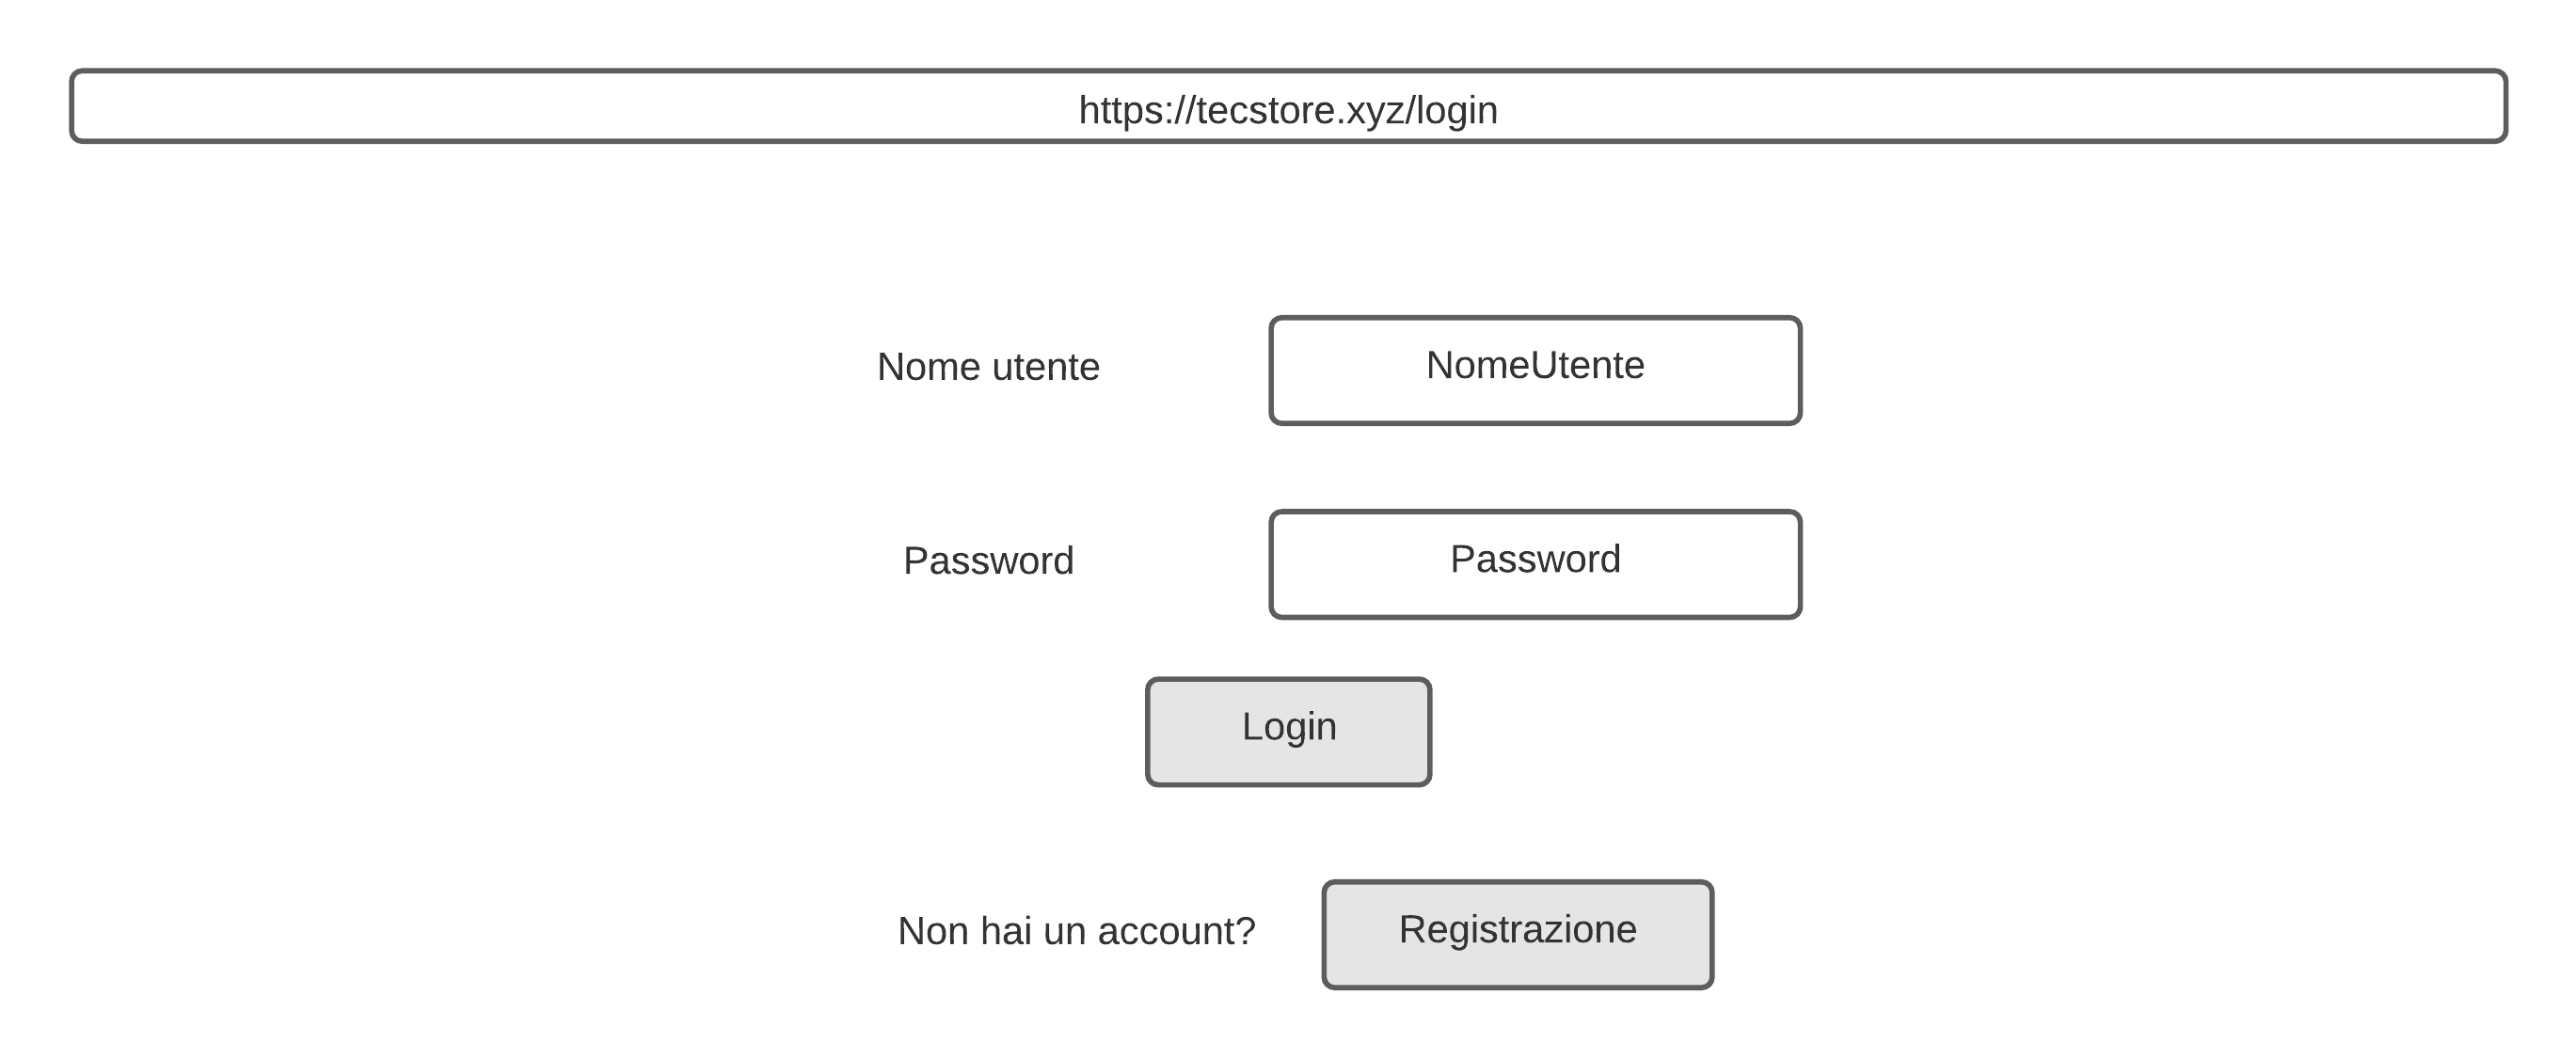
\includegraphics[height=150px]{login}

\item Inserisce quindi i suoi dati nel form, "Luca" in nome, "Garibaldi" in cognome, "lucagaribaldi@email.tld" in email, "password1" in password e in conferma password, "20/06/1991" nel campo data di nascita e fa click sul tasto "Conferma". \\

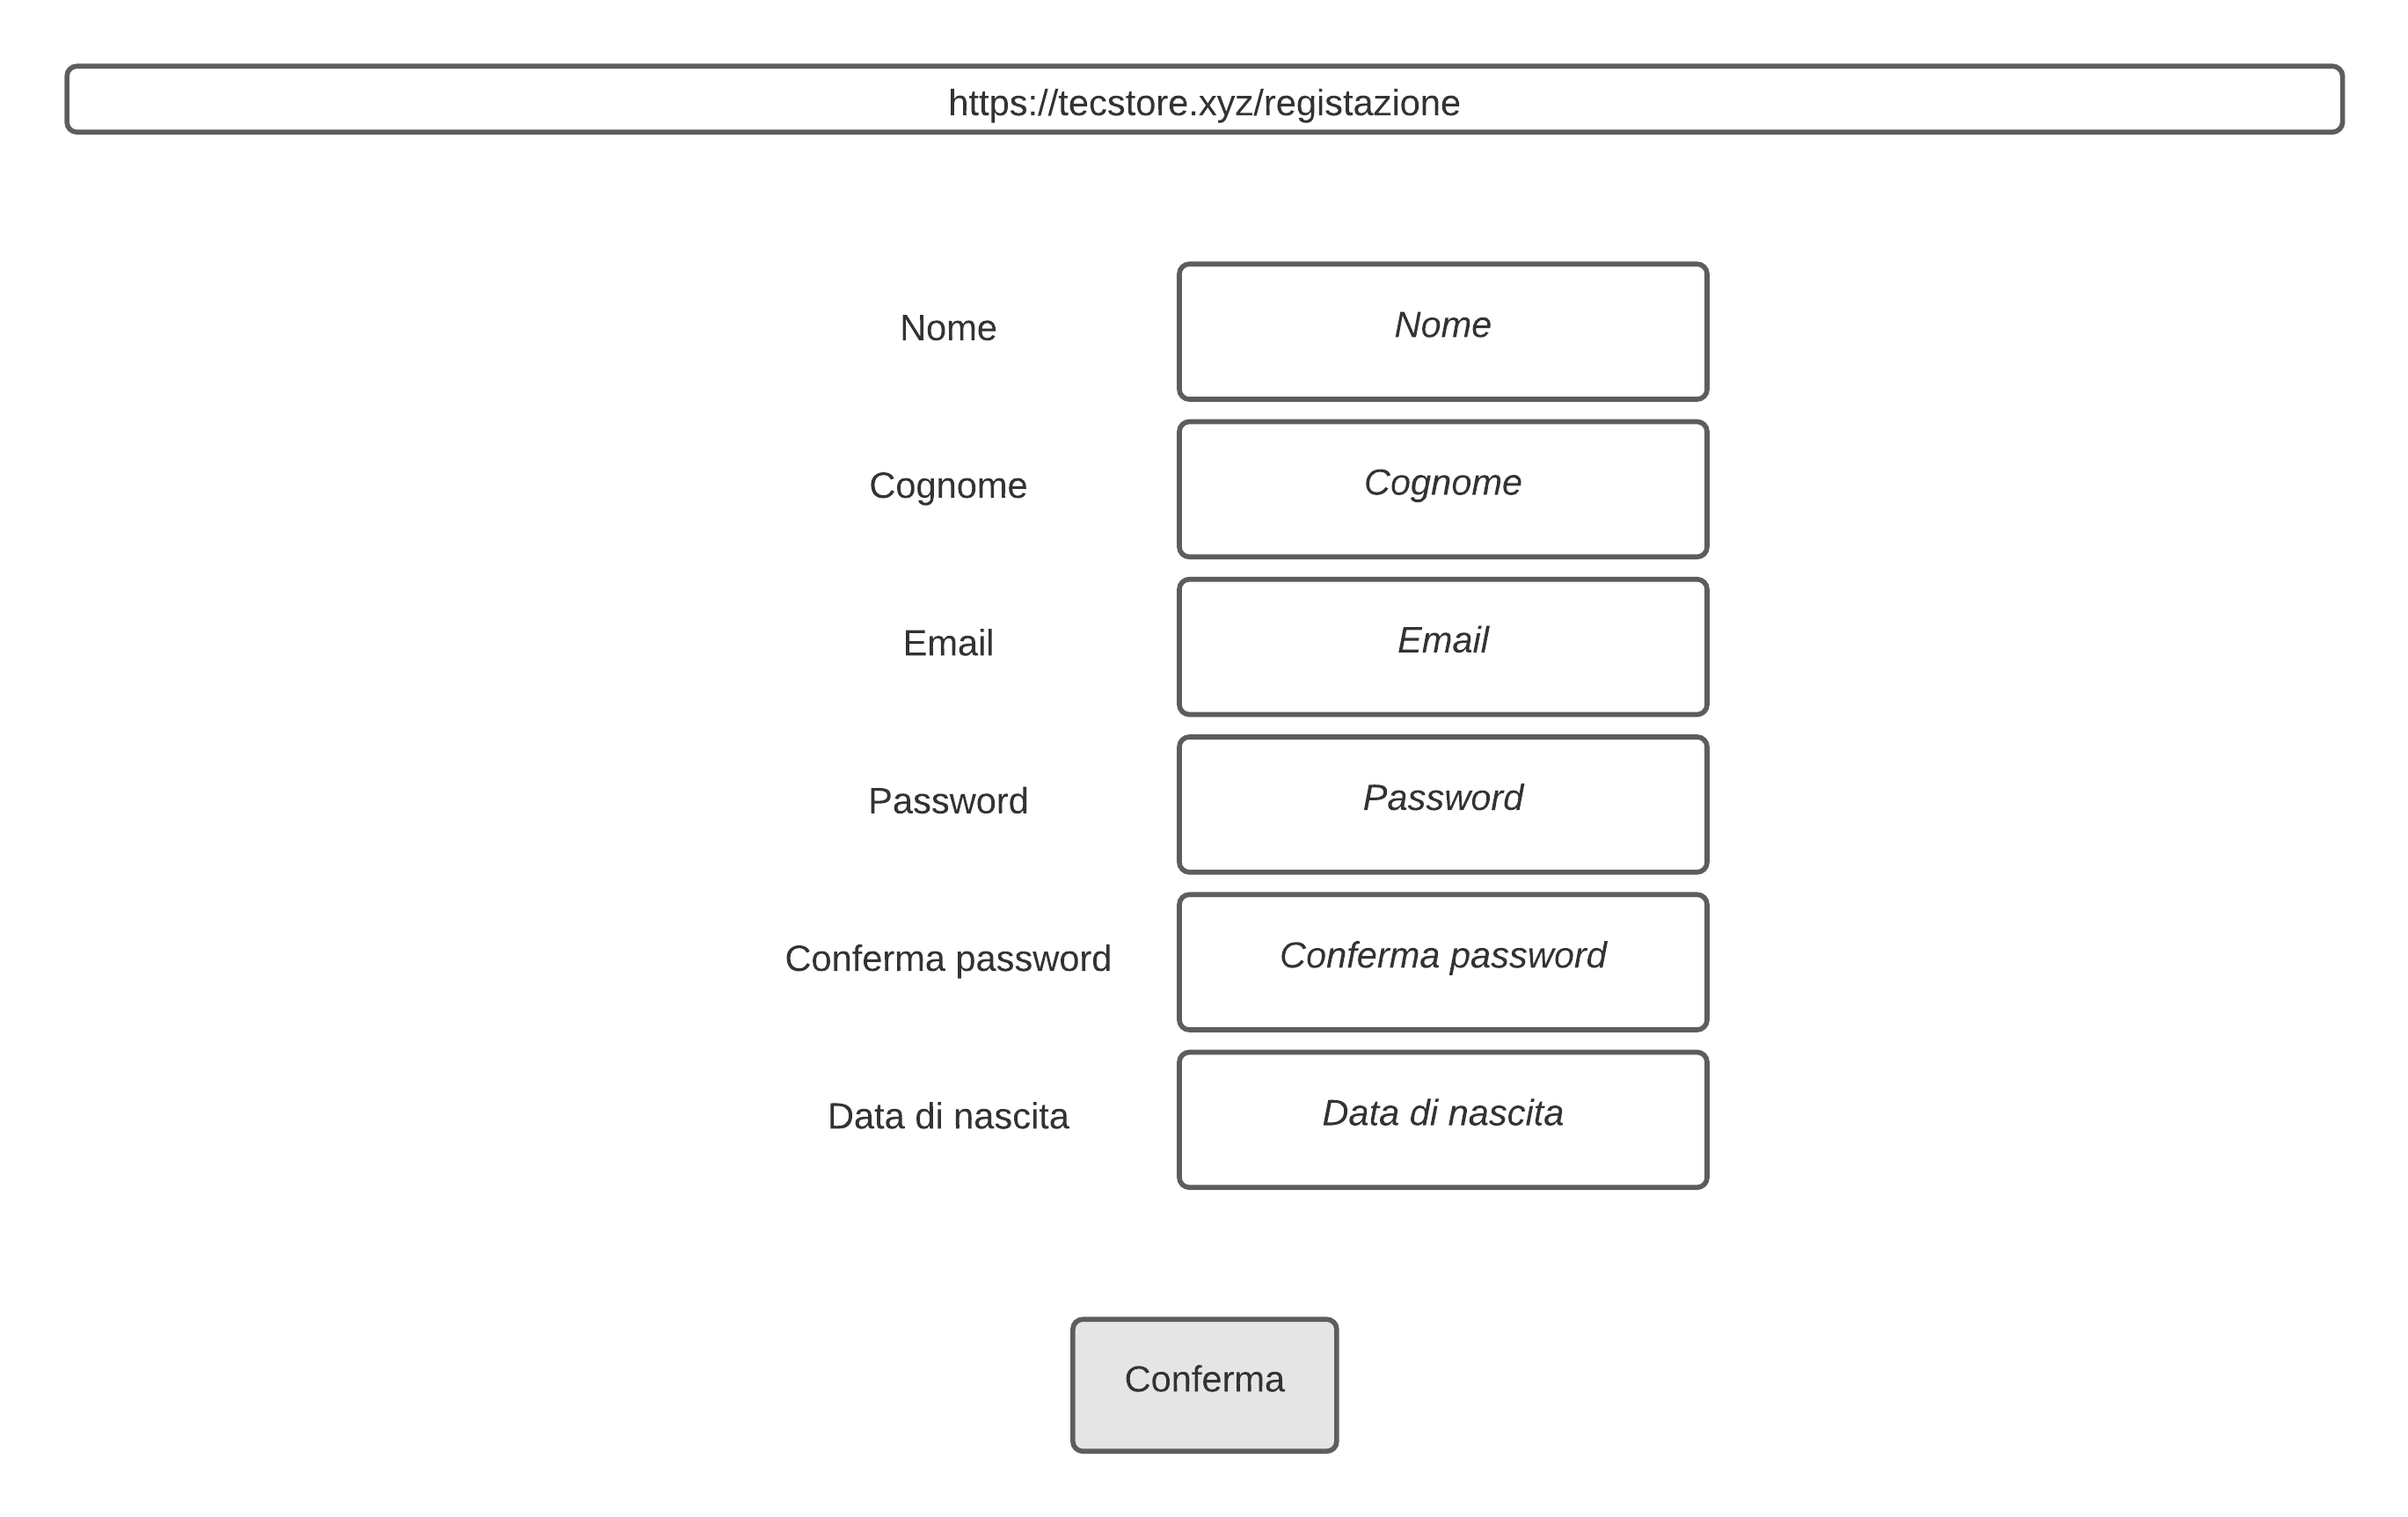
\includegraphics[width=\textwidth]{anagrafica}

\newpage
\item Gli vengono chiesti i dati della carta di credito e inserisce "4555133720756196" nel campo numero, 03/23 nel campo scadenza, 356 nel campo CVV, "Via Roma 1" nel campo indirizzo, "Torino 10123" nel campo città, e "Italia" nel campo nazione e fa click sul tasto "Conferma".

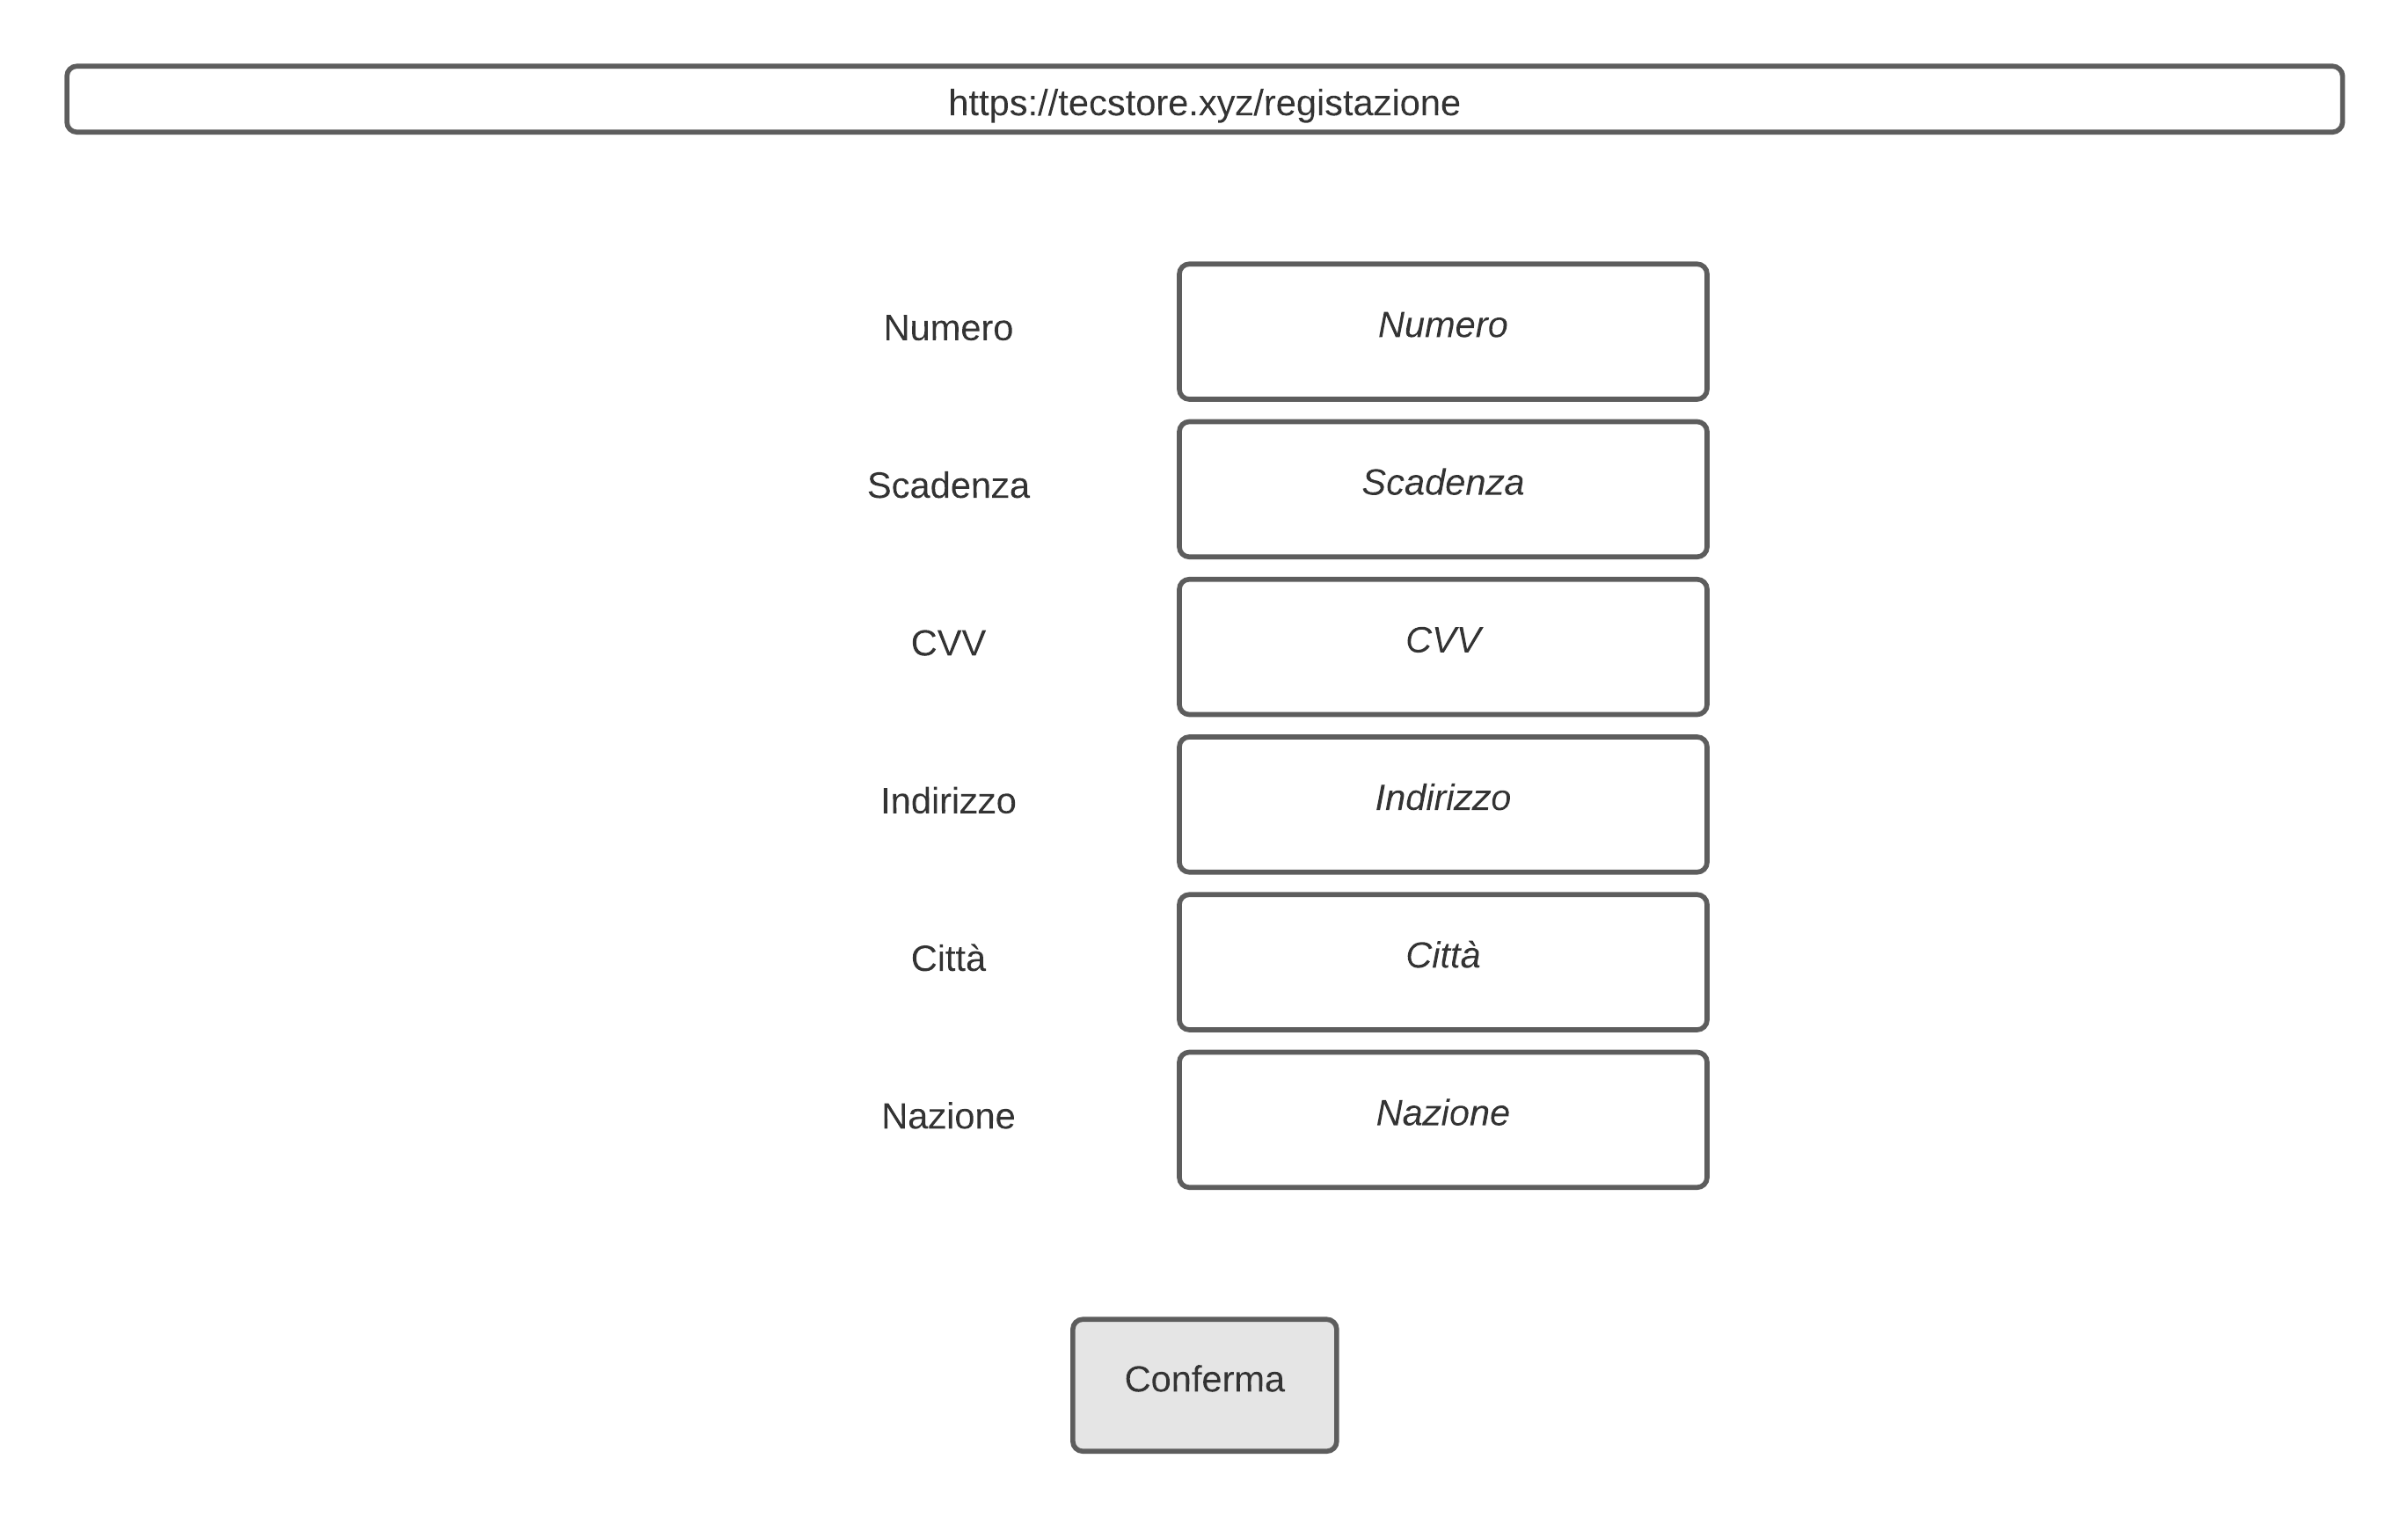
\includegraphics[width=\textwidth]{carta}

\item Gli viene chiesta un'ultima conferma prima di effettuare l'ordine. \\
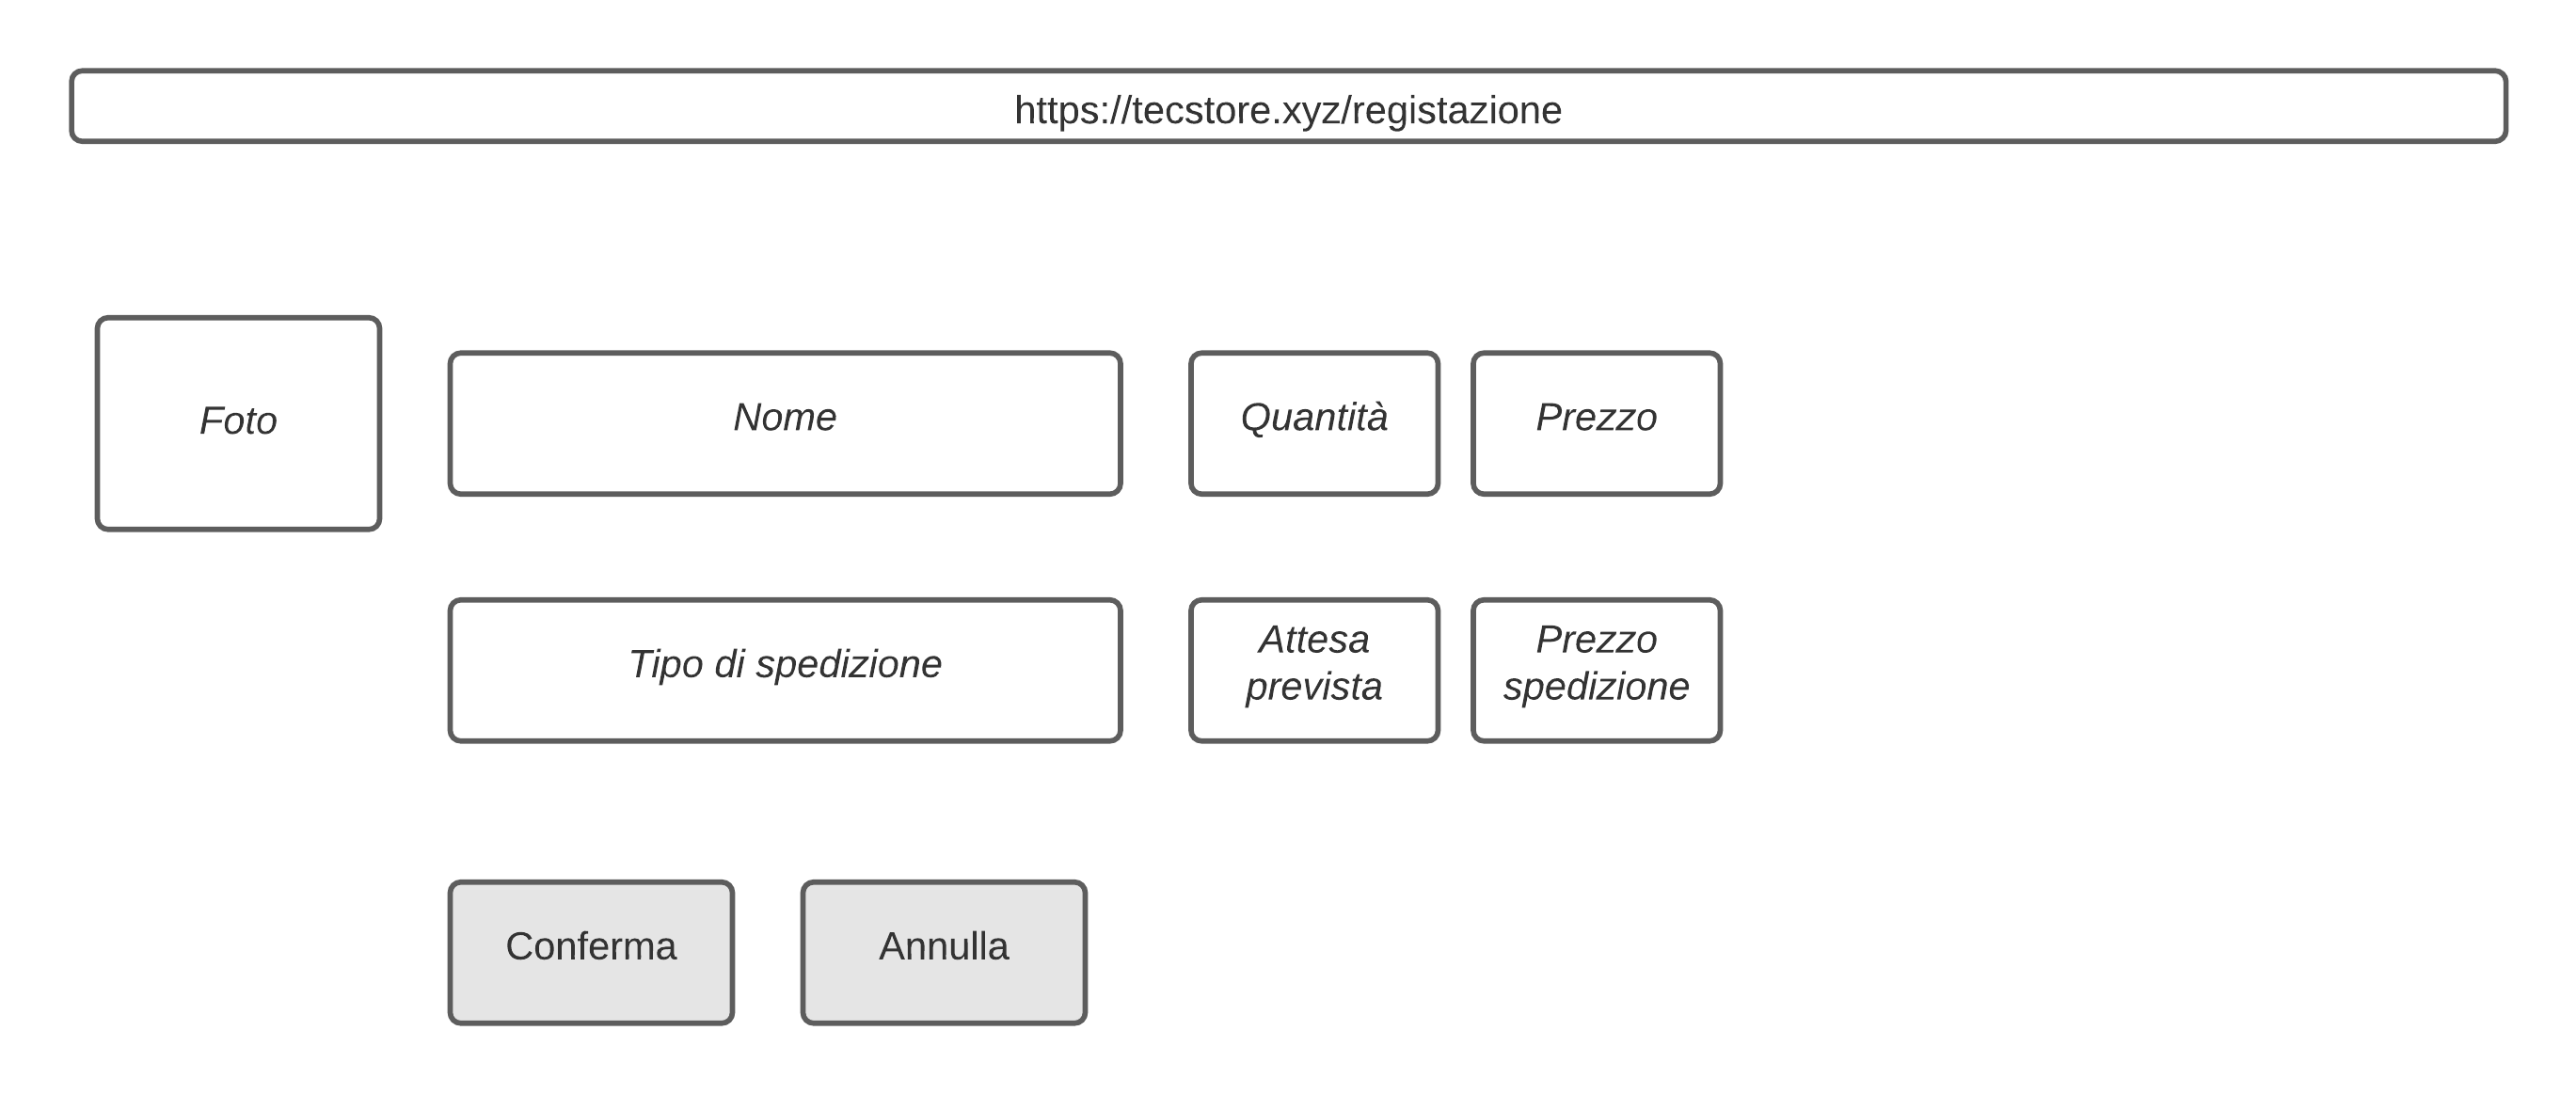
\includegraphics[width=\textwidth]{conferma}

\item Al che Luca preme "Acquista".

\item Il mattino dopo, Massimo arriva al lavoro, effettua il login alla pagina riservata al magazzino con le credenziali "magazz1" e "0GfbwmXYCIERGT3aU7ja" come password. Vede l'ordine effettuato da Luca, reperisce l'articolo dal magazzino, lo impacchetta, stampa la bolla di spedizione e prenota il corriere per il ritiro dell'articolo.

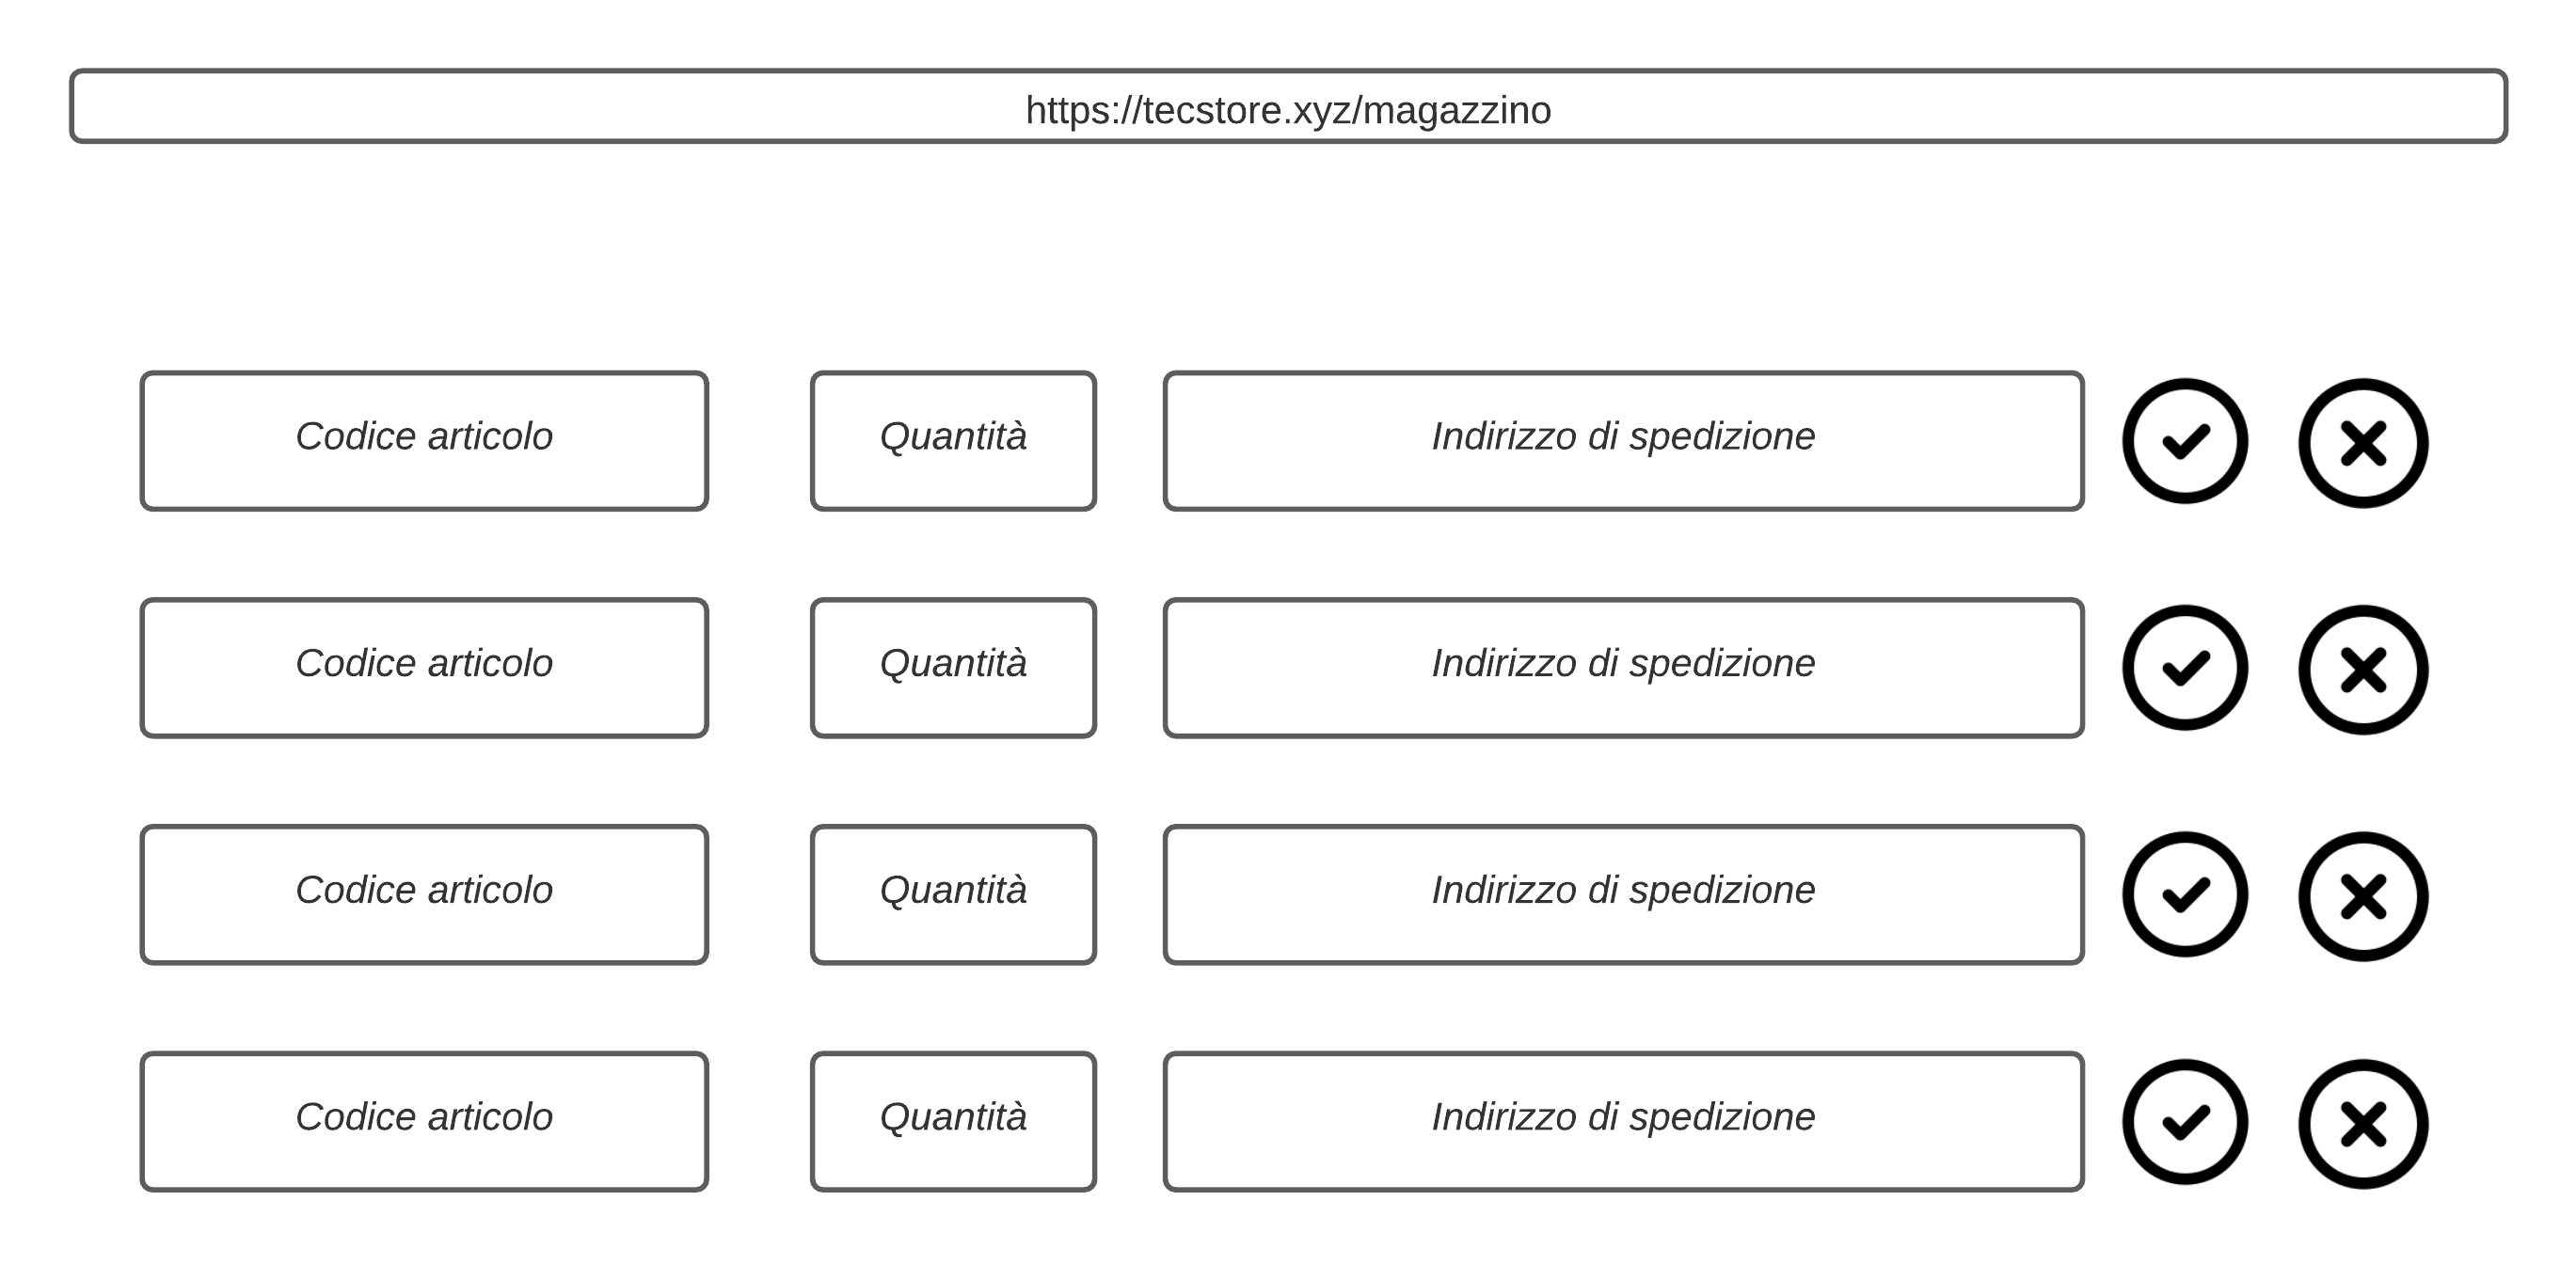
\includegraphics[width=\textwidth]{magazzino}

\item Tre giorni dopo un corriere gli consegna l'articolo acquistato.
\end{enumerate}

\newpage
\subsection{Un utente apre una segnalazione all'assistenza}
\textbf{Attori:} Carlo Cavour, utente e Lucia Pellegrino, centralinista \\
\noindent
\textbf{Flusso di eventi:}
\begin{enumerate}
\item 10 giorni fa Carlo ha ordinato un nuovo hard disk, ma non l'ha ancora ricevuto. Decide quindi di aprire un ticket su TecStore.

\item Apre la homepage del sito. \\

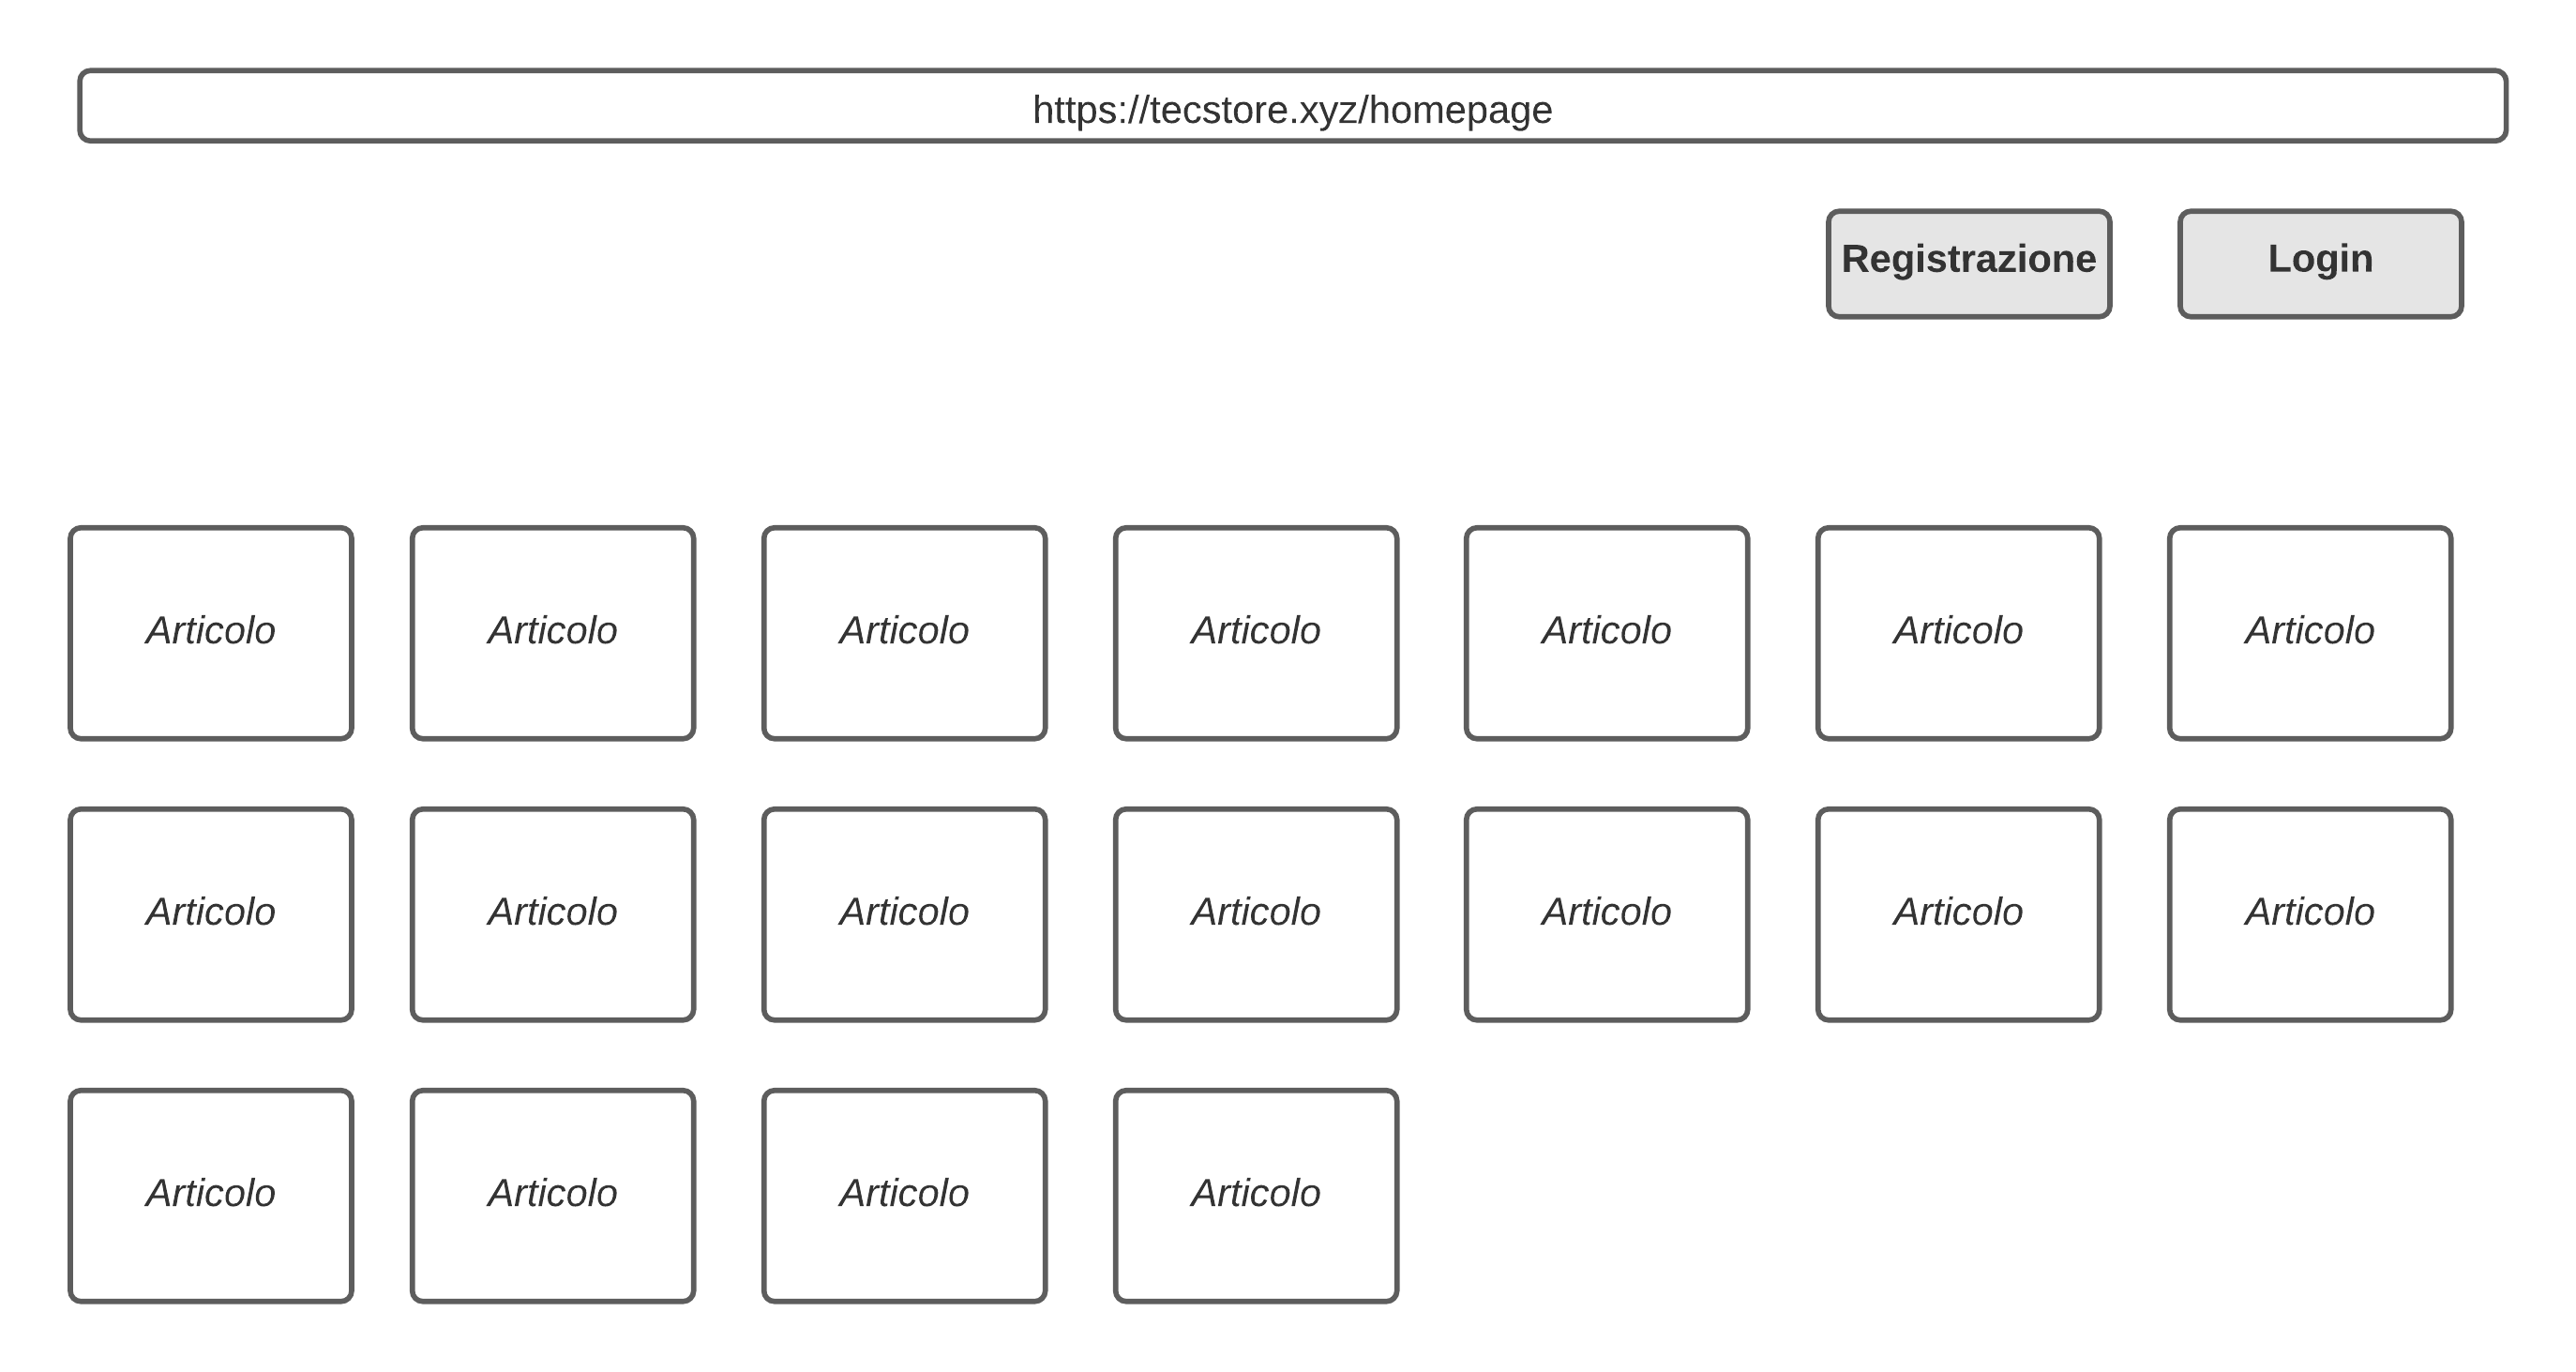
\includegraphics[width=\textwidth]{homepage}

\item Fa click sul tasto "Login" e viene riportato al form in cui gli viene chiesto di inserire email e password, inserisce rispettivamente \\ "carlocavour@email.tld" e "hunter2" e fa click sul tasto per confermare.

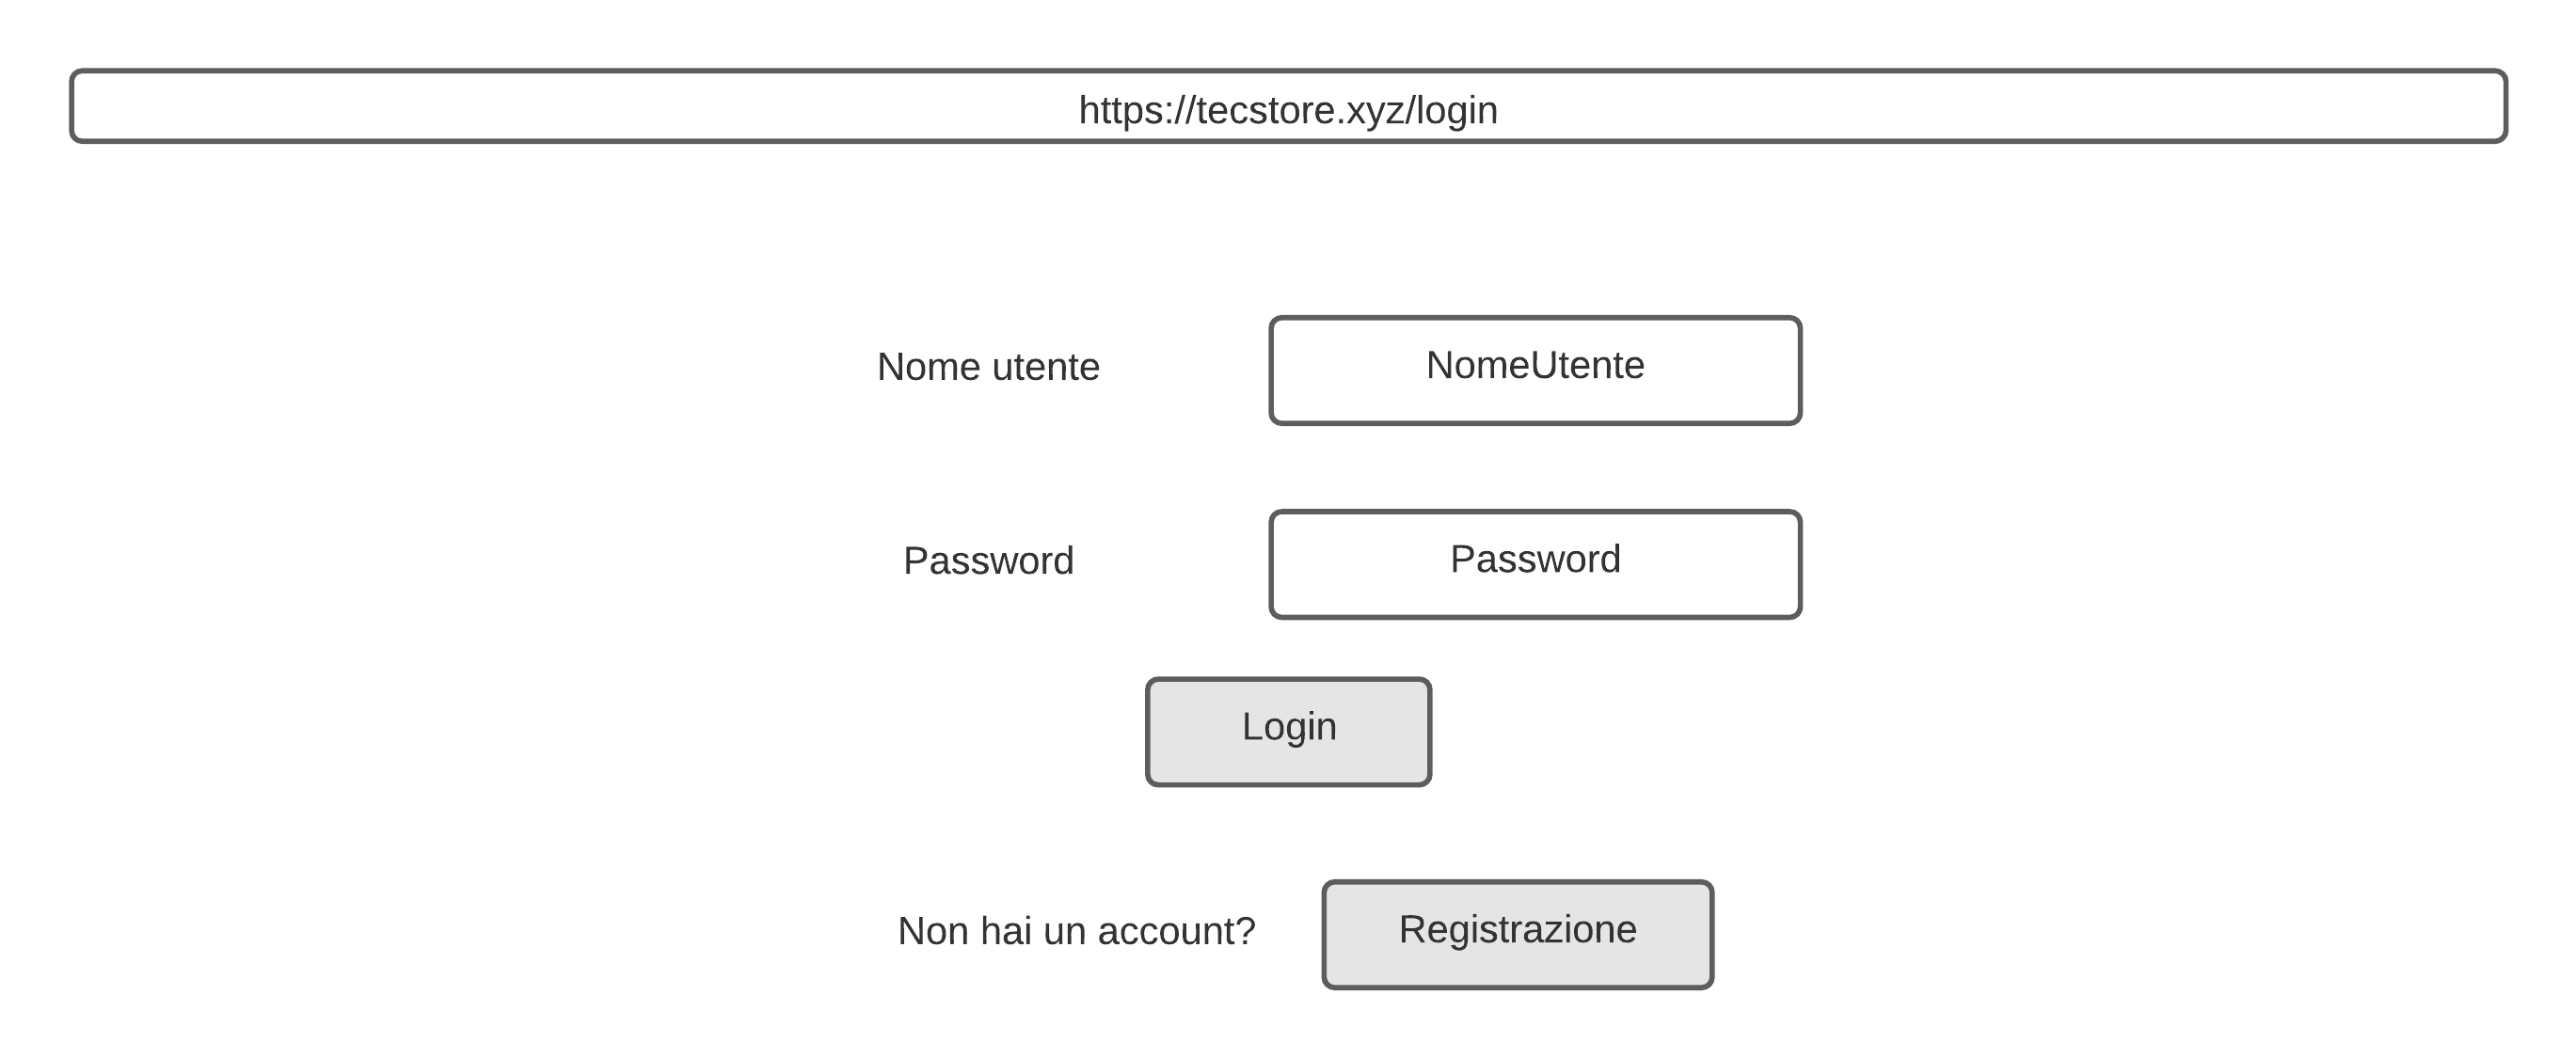
\includegraphics[height=150px]{login}

\newpage
\item Viene quindi reindirizzato all'interfaccia principale. Passa il mouse sul suo nome e fa click sul tasto "Assistenza clienti".

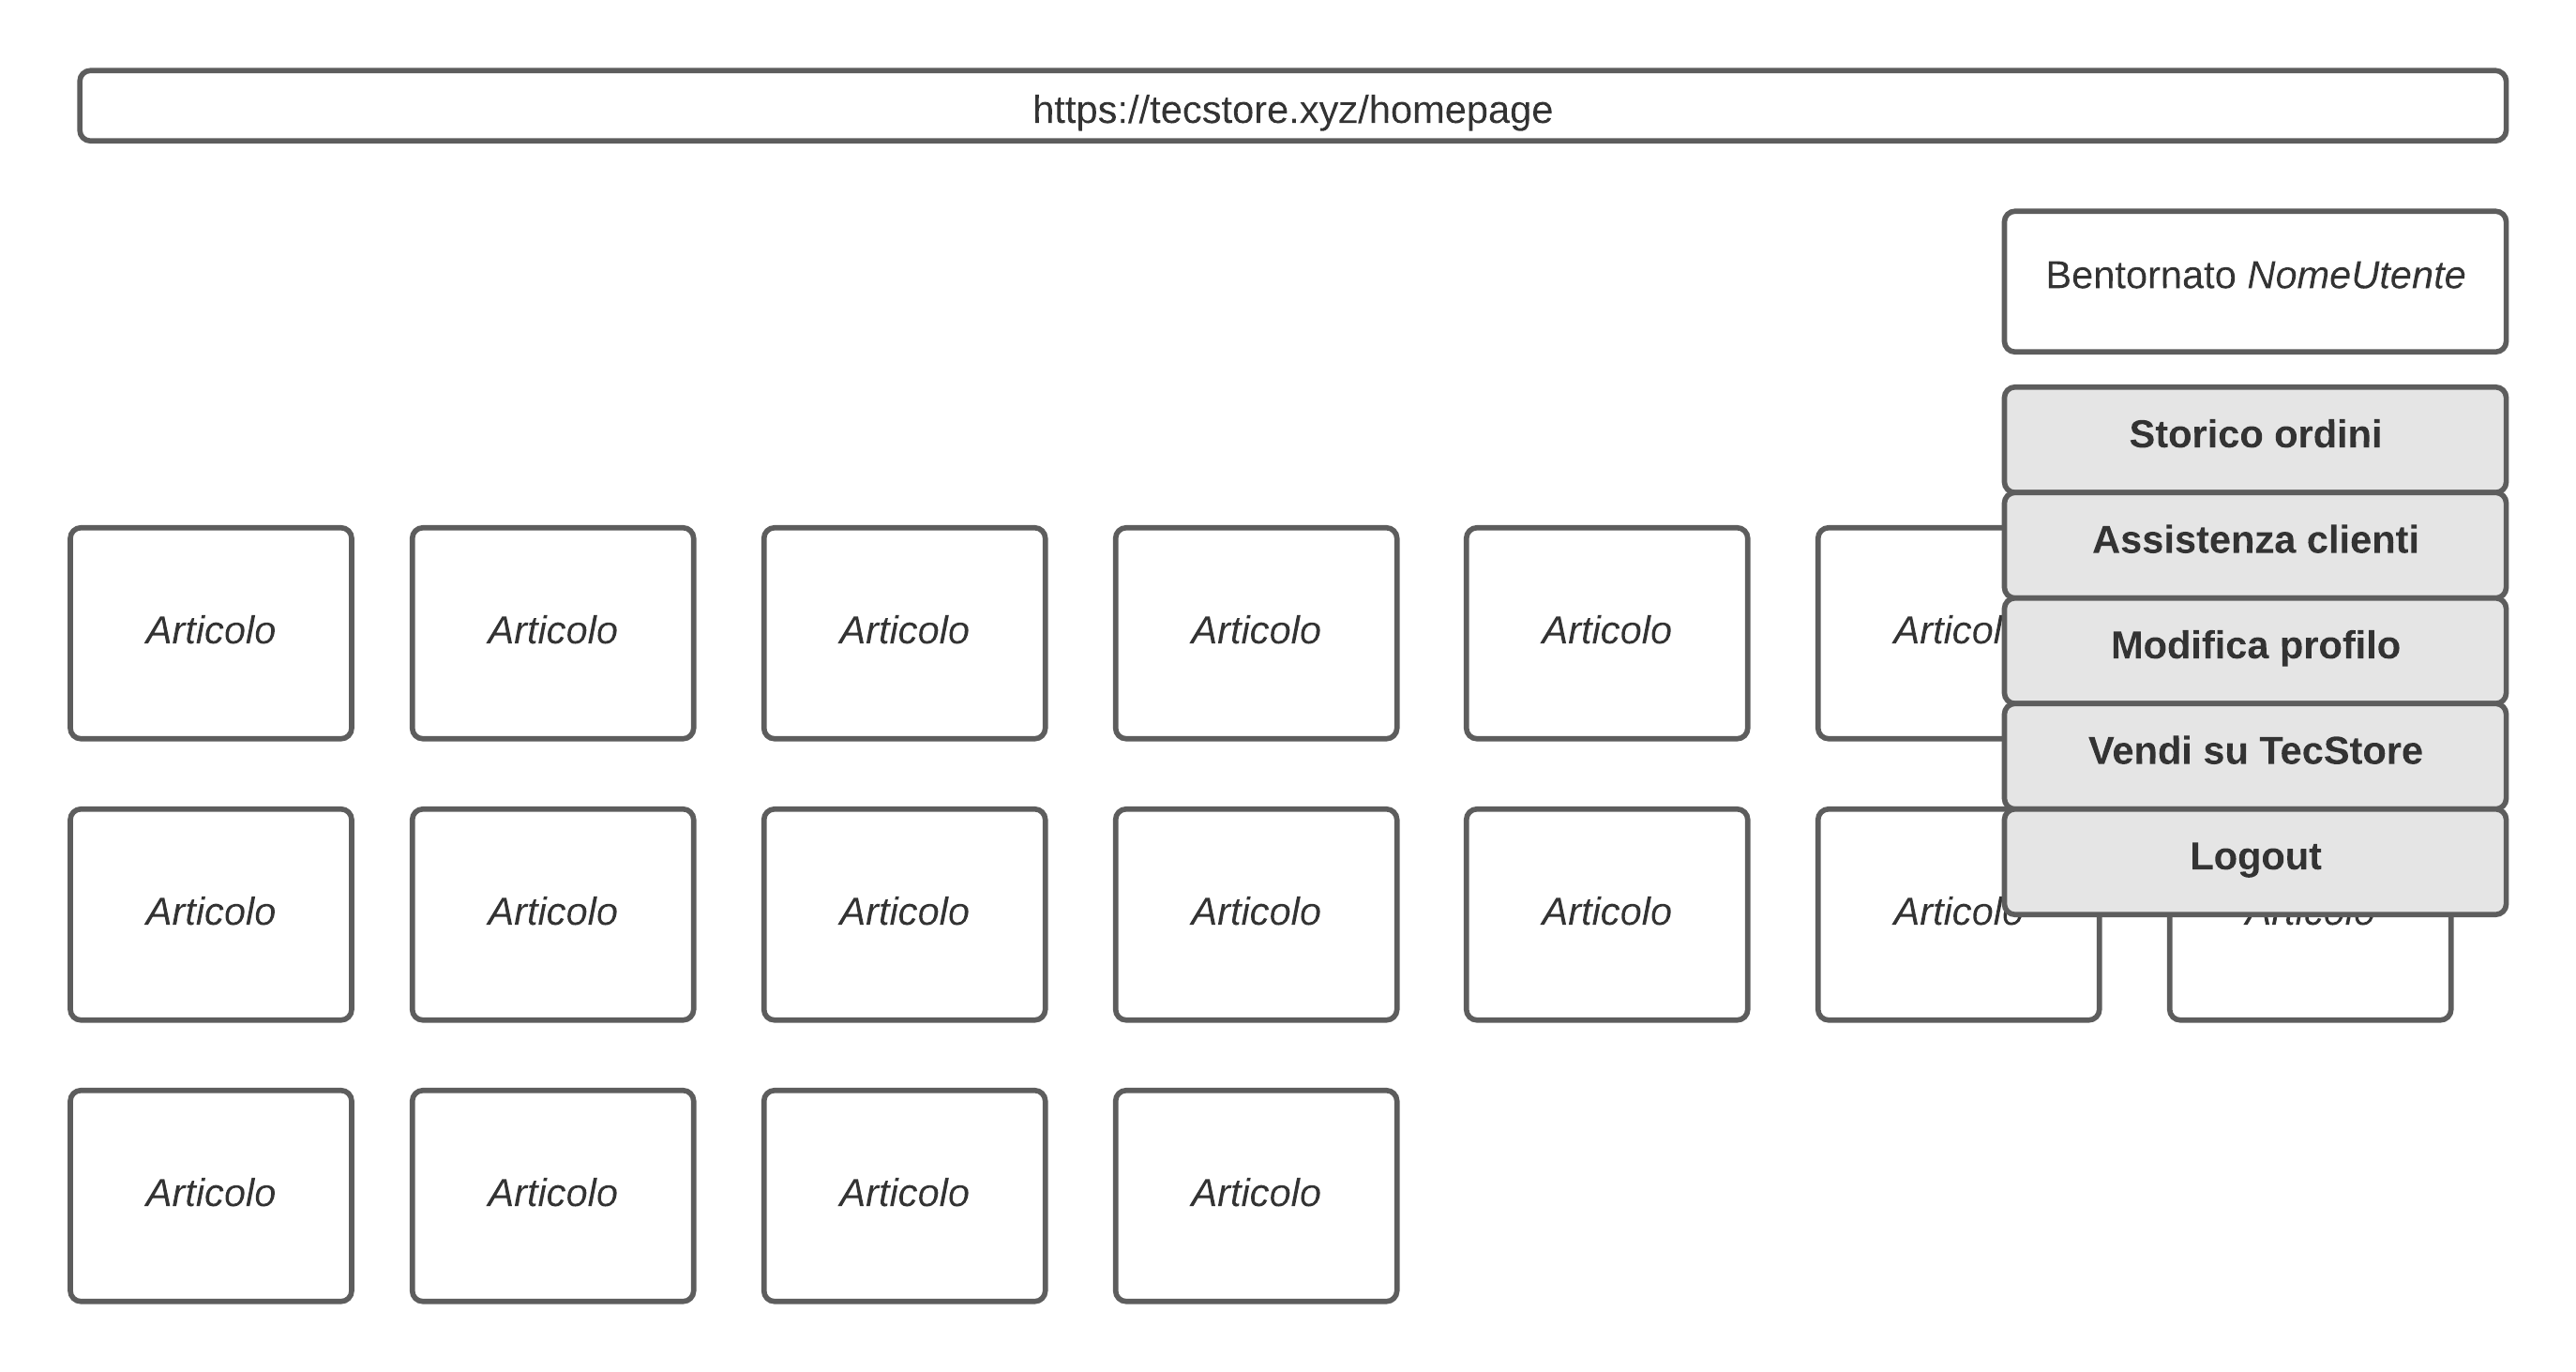
\includegraphics[width=\textwidth]{homepage_login}

\item Viene portato nella pagina per la creazione di un nuovo ticket, sceglie "Problemi di spedizione" come tipologia e scrive "Non ho ricevuto il mio articolo dopo 10 giorni" nel campo descrizione. \\
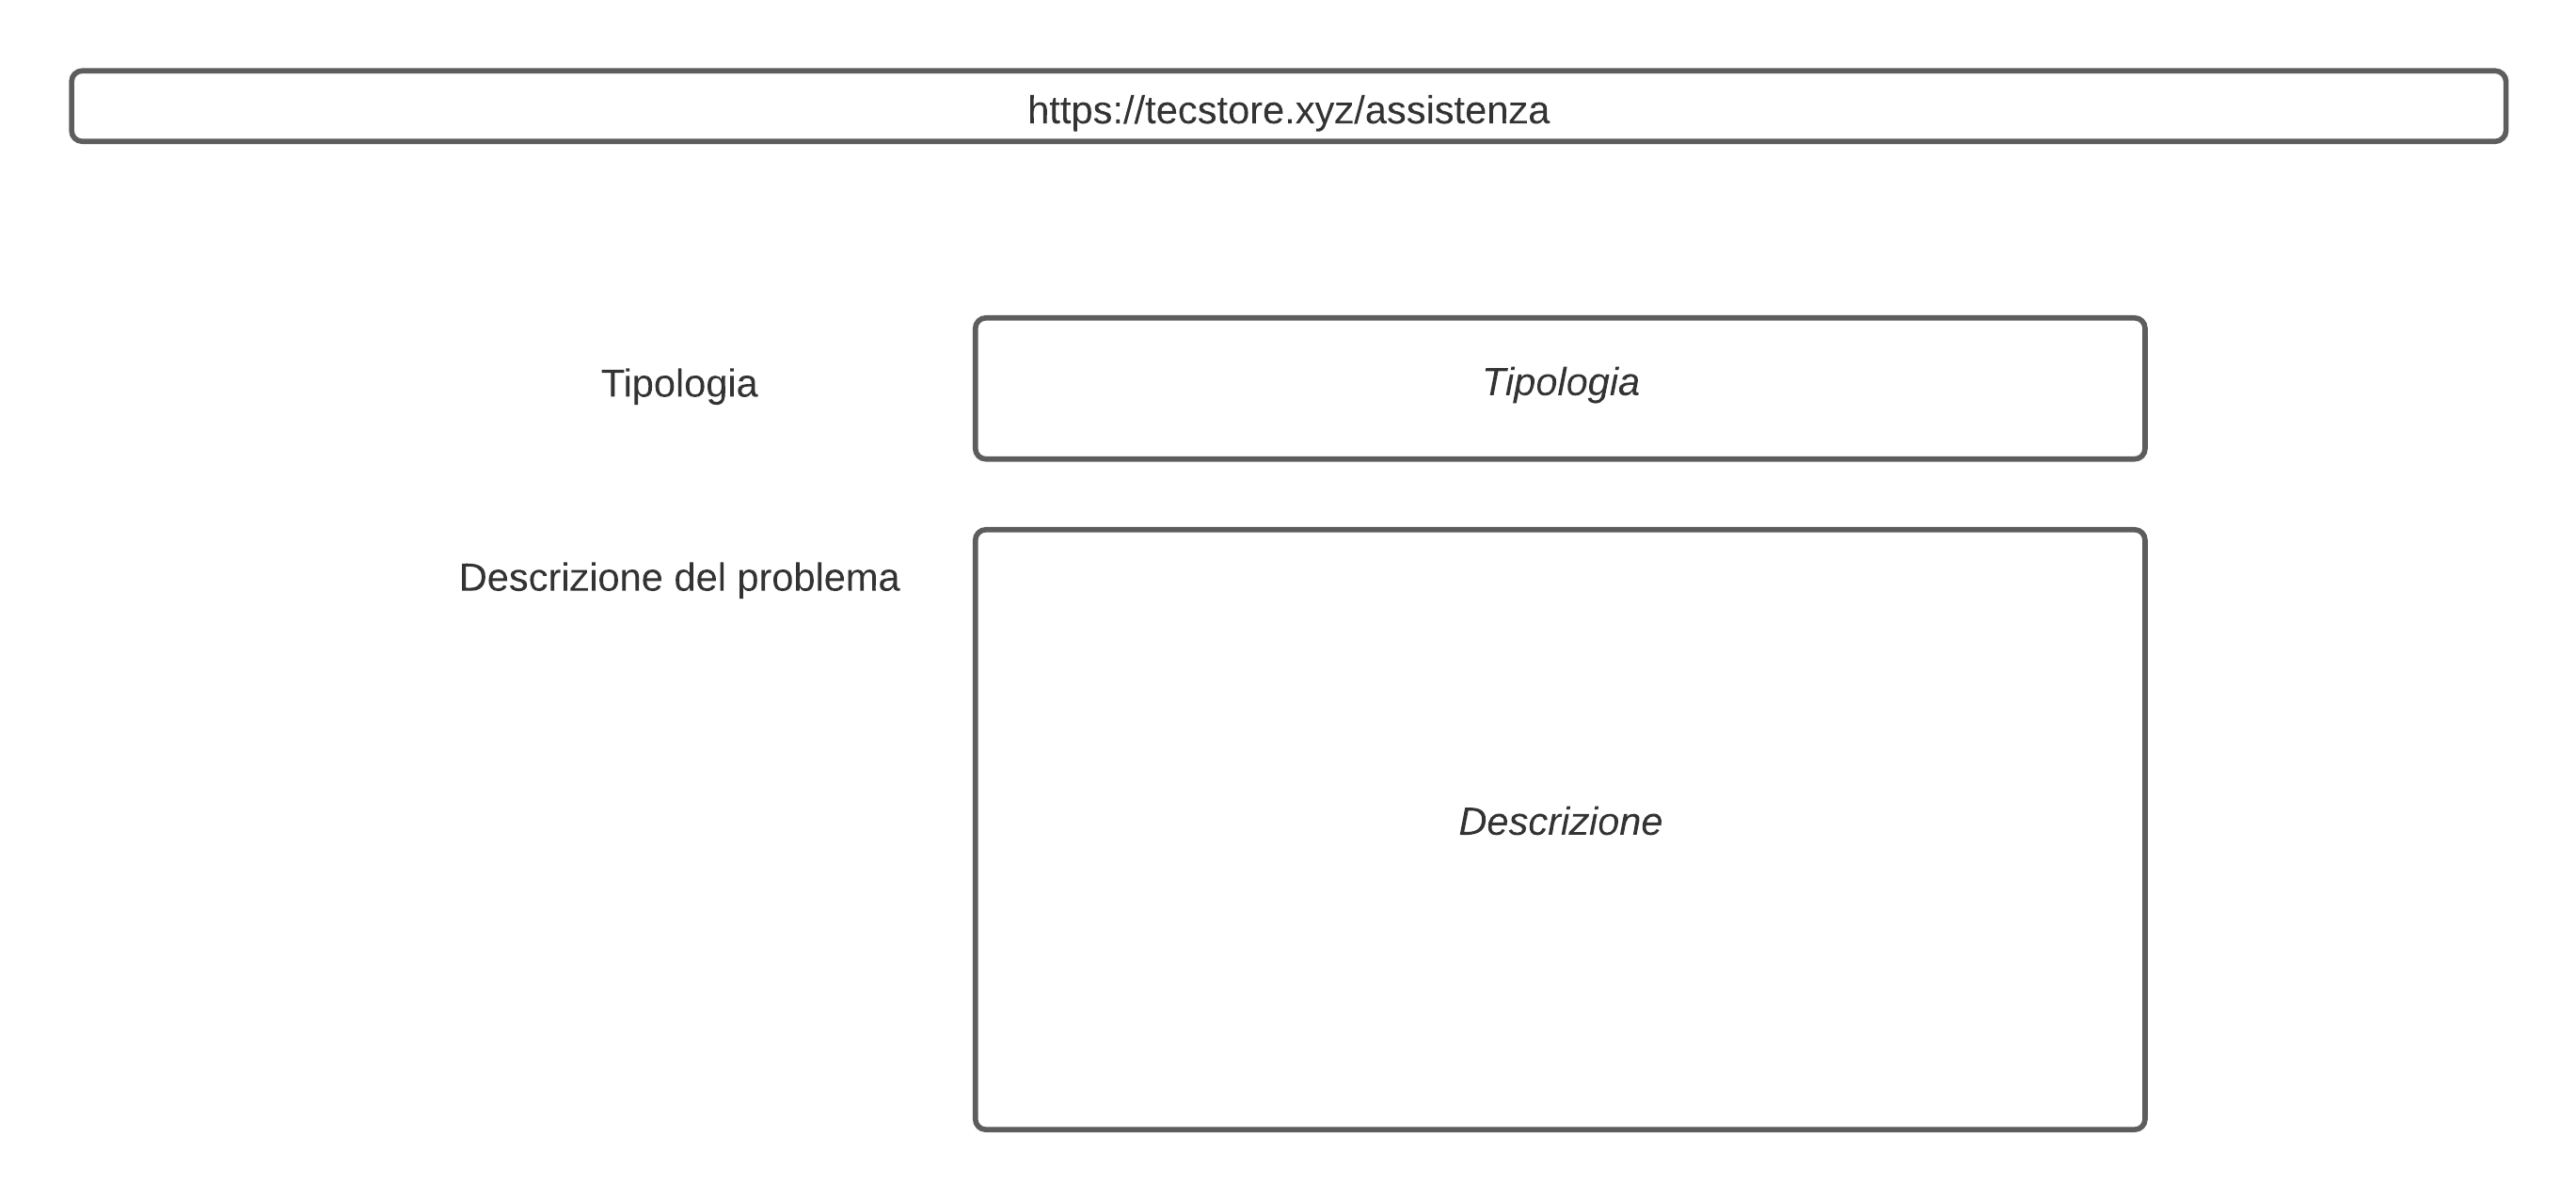
\includegraphics[width=\textwidth]{assistenza}

\newpage
\item Lucia effettua il login alla pagina riservata all'assistenza, vede il nuovo ticket e risponde a Carlo che nei giorni precedenti ci sono stati problemi con il corriere che TecStore solitamente utilizza per spedire gli articoli e lo assicura che riceverà l'articolo entro le successive 48 ore.

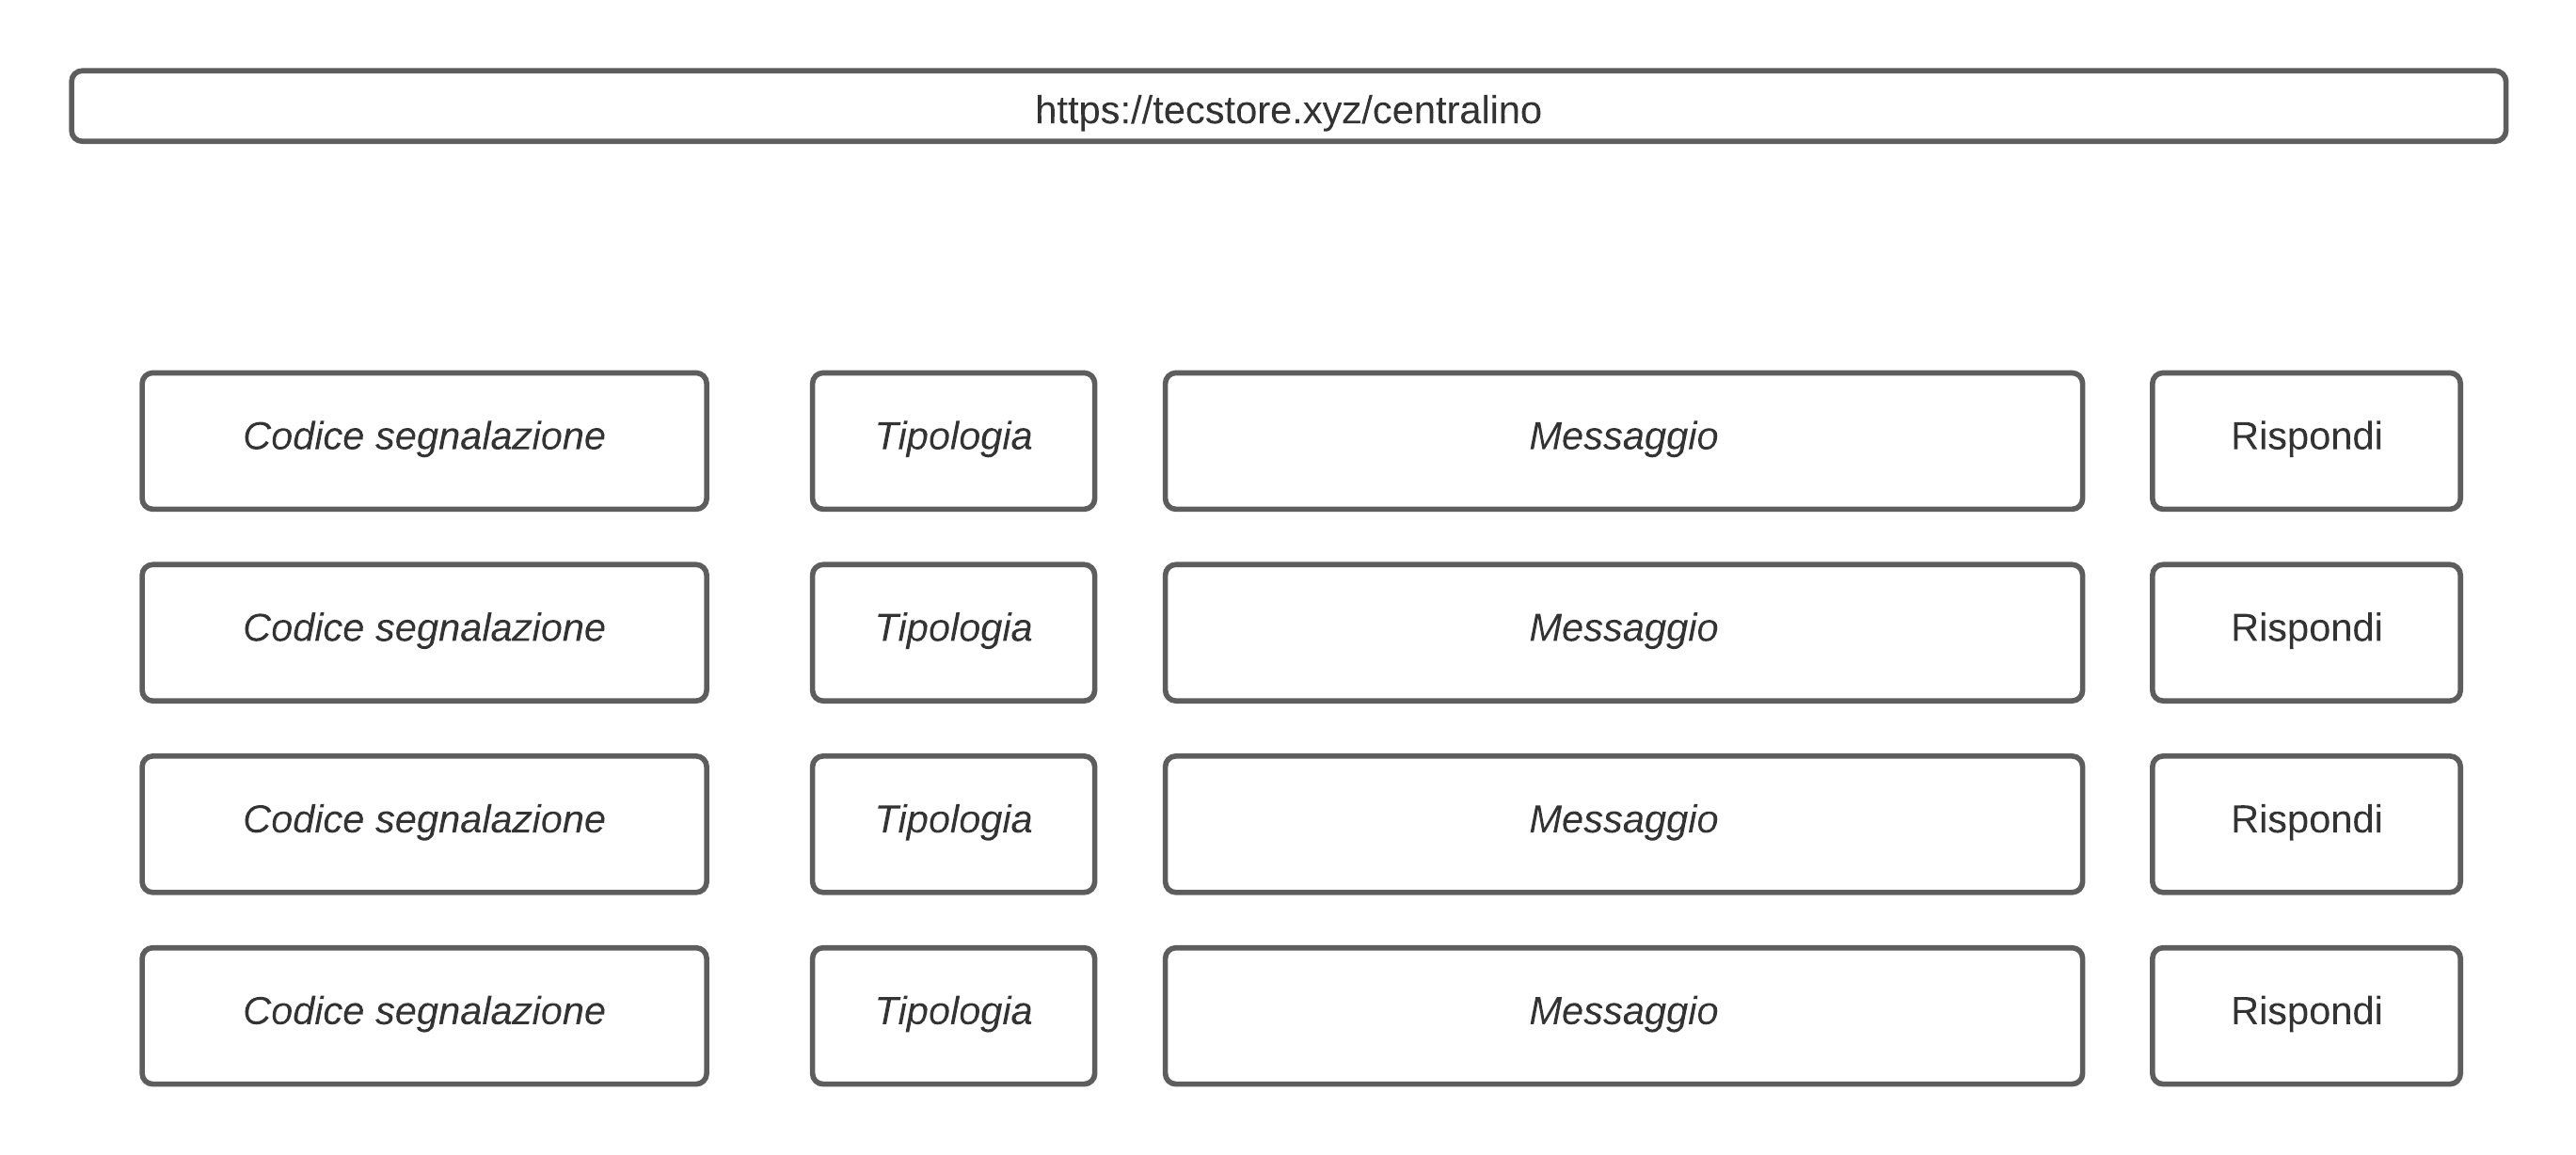
\includegraphics[width=\textwidth]{centralino}

\item La mattina del giorno dopo Carlo riceve l'articolo ordinato.
\end{enumerate}

\subsection{Un utente vuole mettere in vendita un articolo}
\textbf{Attori:} Alfonso Siciliani, utente e Silvana Piazza, centralinista \\

\noindent
\textbf{Flusso di eventi:}

\begin{enumerate}

\item Alfonso ha un piccolo negozio di informatica e ha un surplus di monitor che non riesce a vendere nel suo negozio. Decide quindi di metterli in vendita online.

\item Per ampliare la potenziale utenza, oltre a piattaforme più note, decide di inserirlo anche in qualche sito meno conosciuto e sceglie tra le possibili opzioni anche TecStore.
\newpage

\item Essendo un utente già registrato, apre la homepage, clicka sul link "Login".

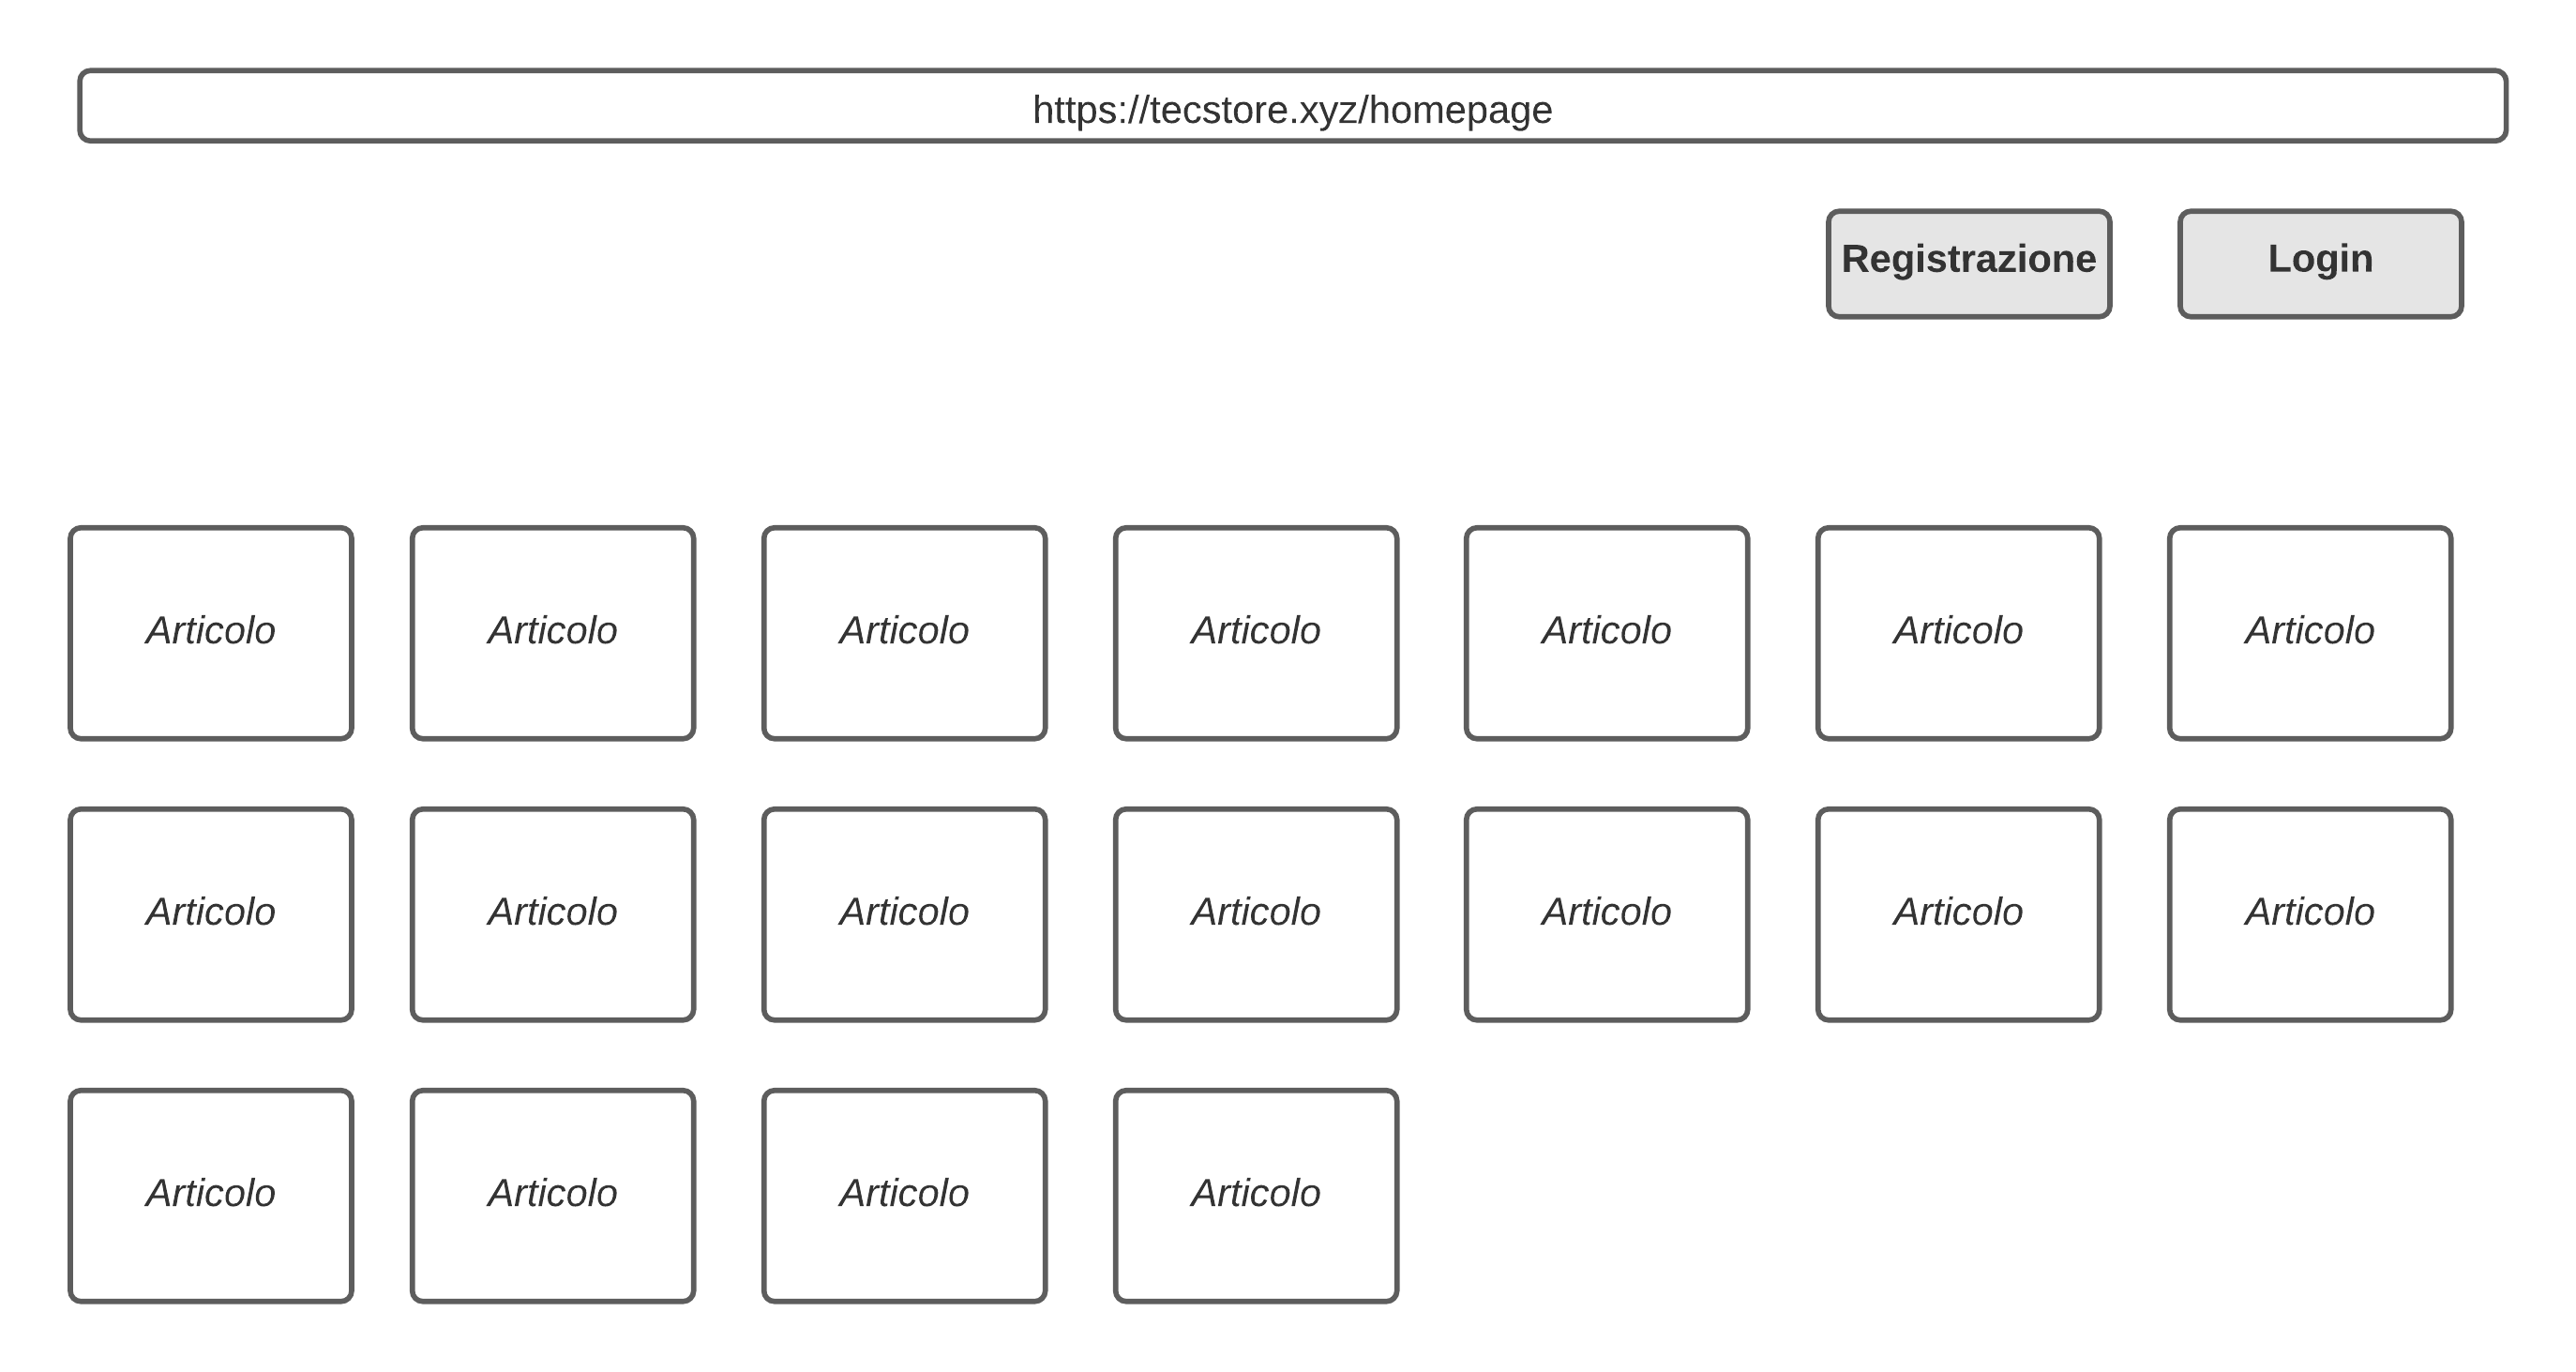
\includegraphics[width=\textwidth]{homepage}

\item Inserisce i suoi dati nel form, rispettivamente "alfonsosiciliani@email.tld" e "KDCH5GeWLBBus02fu6W4"

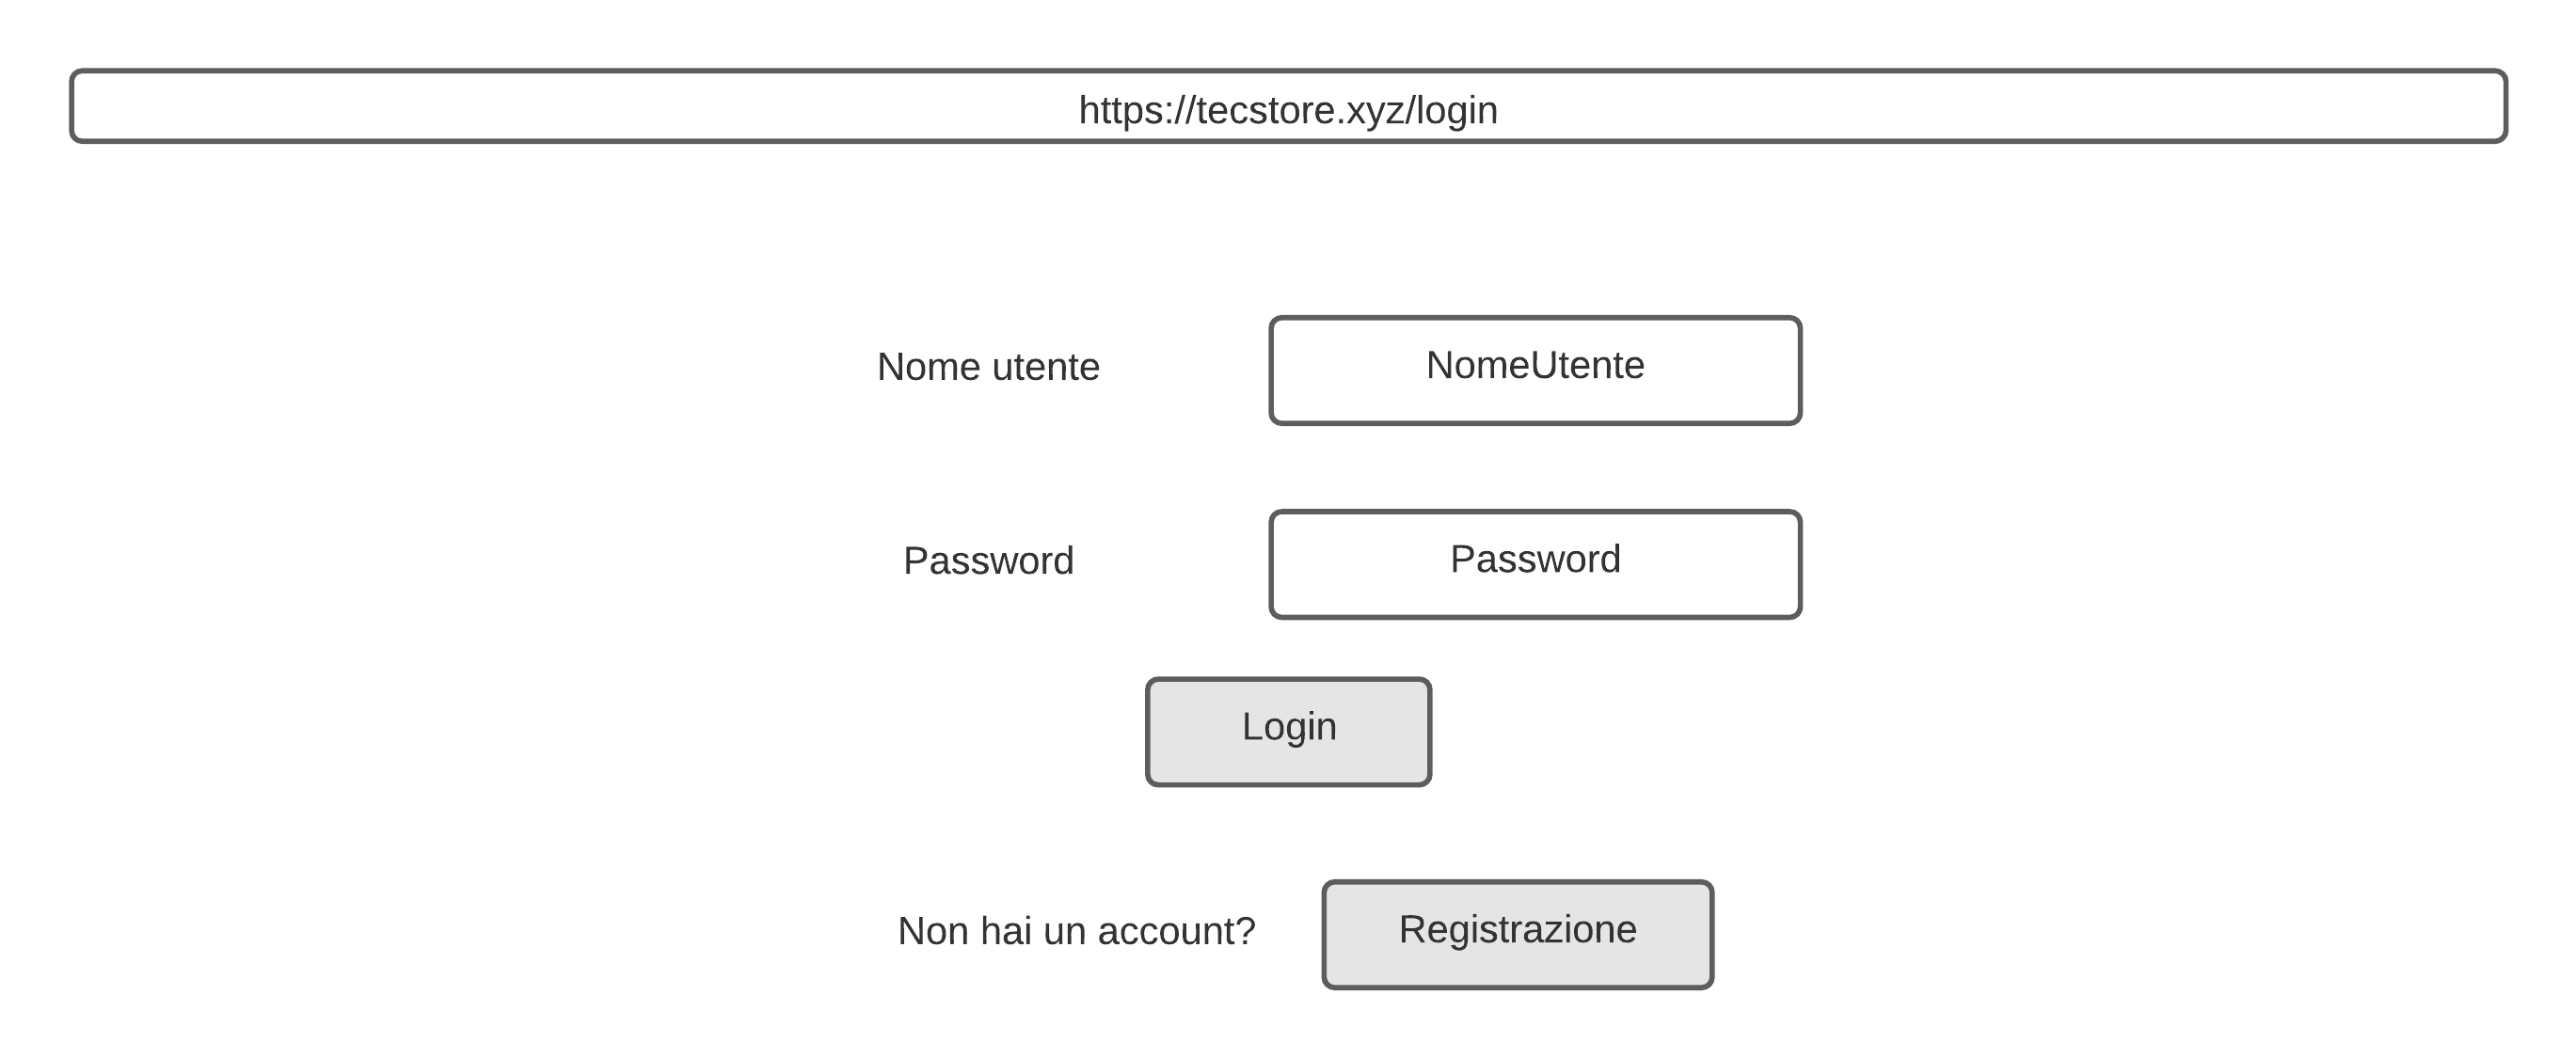
\includegraphics[width=\textwidth]{login}

\newpage

\item Viene quindi reindirizzato alla homepage, passa il mouse sul suo nome e clicka sul link "Vendi su TecStore".

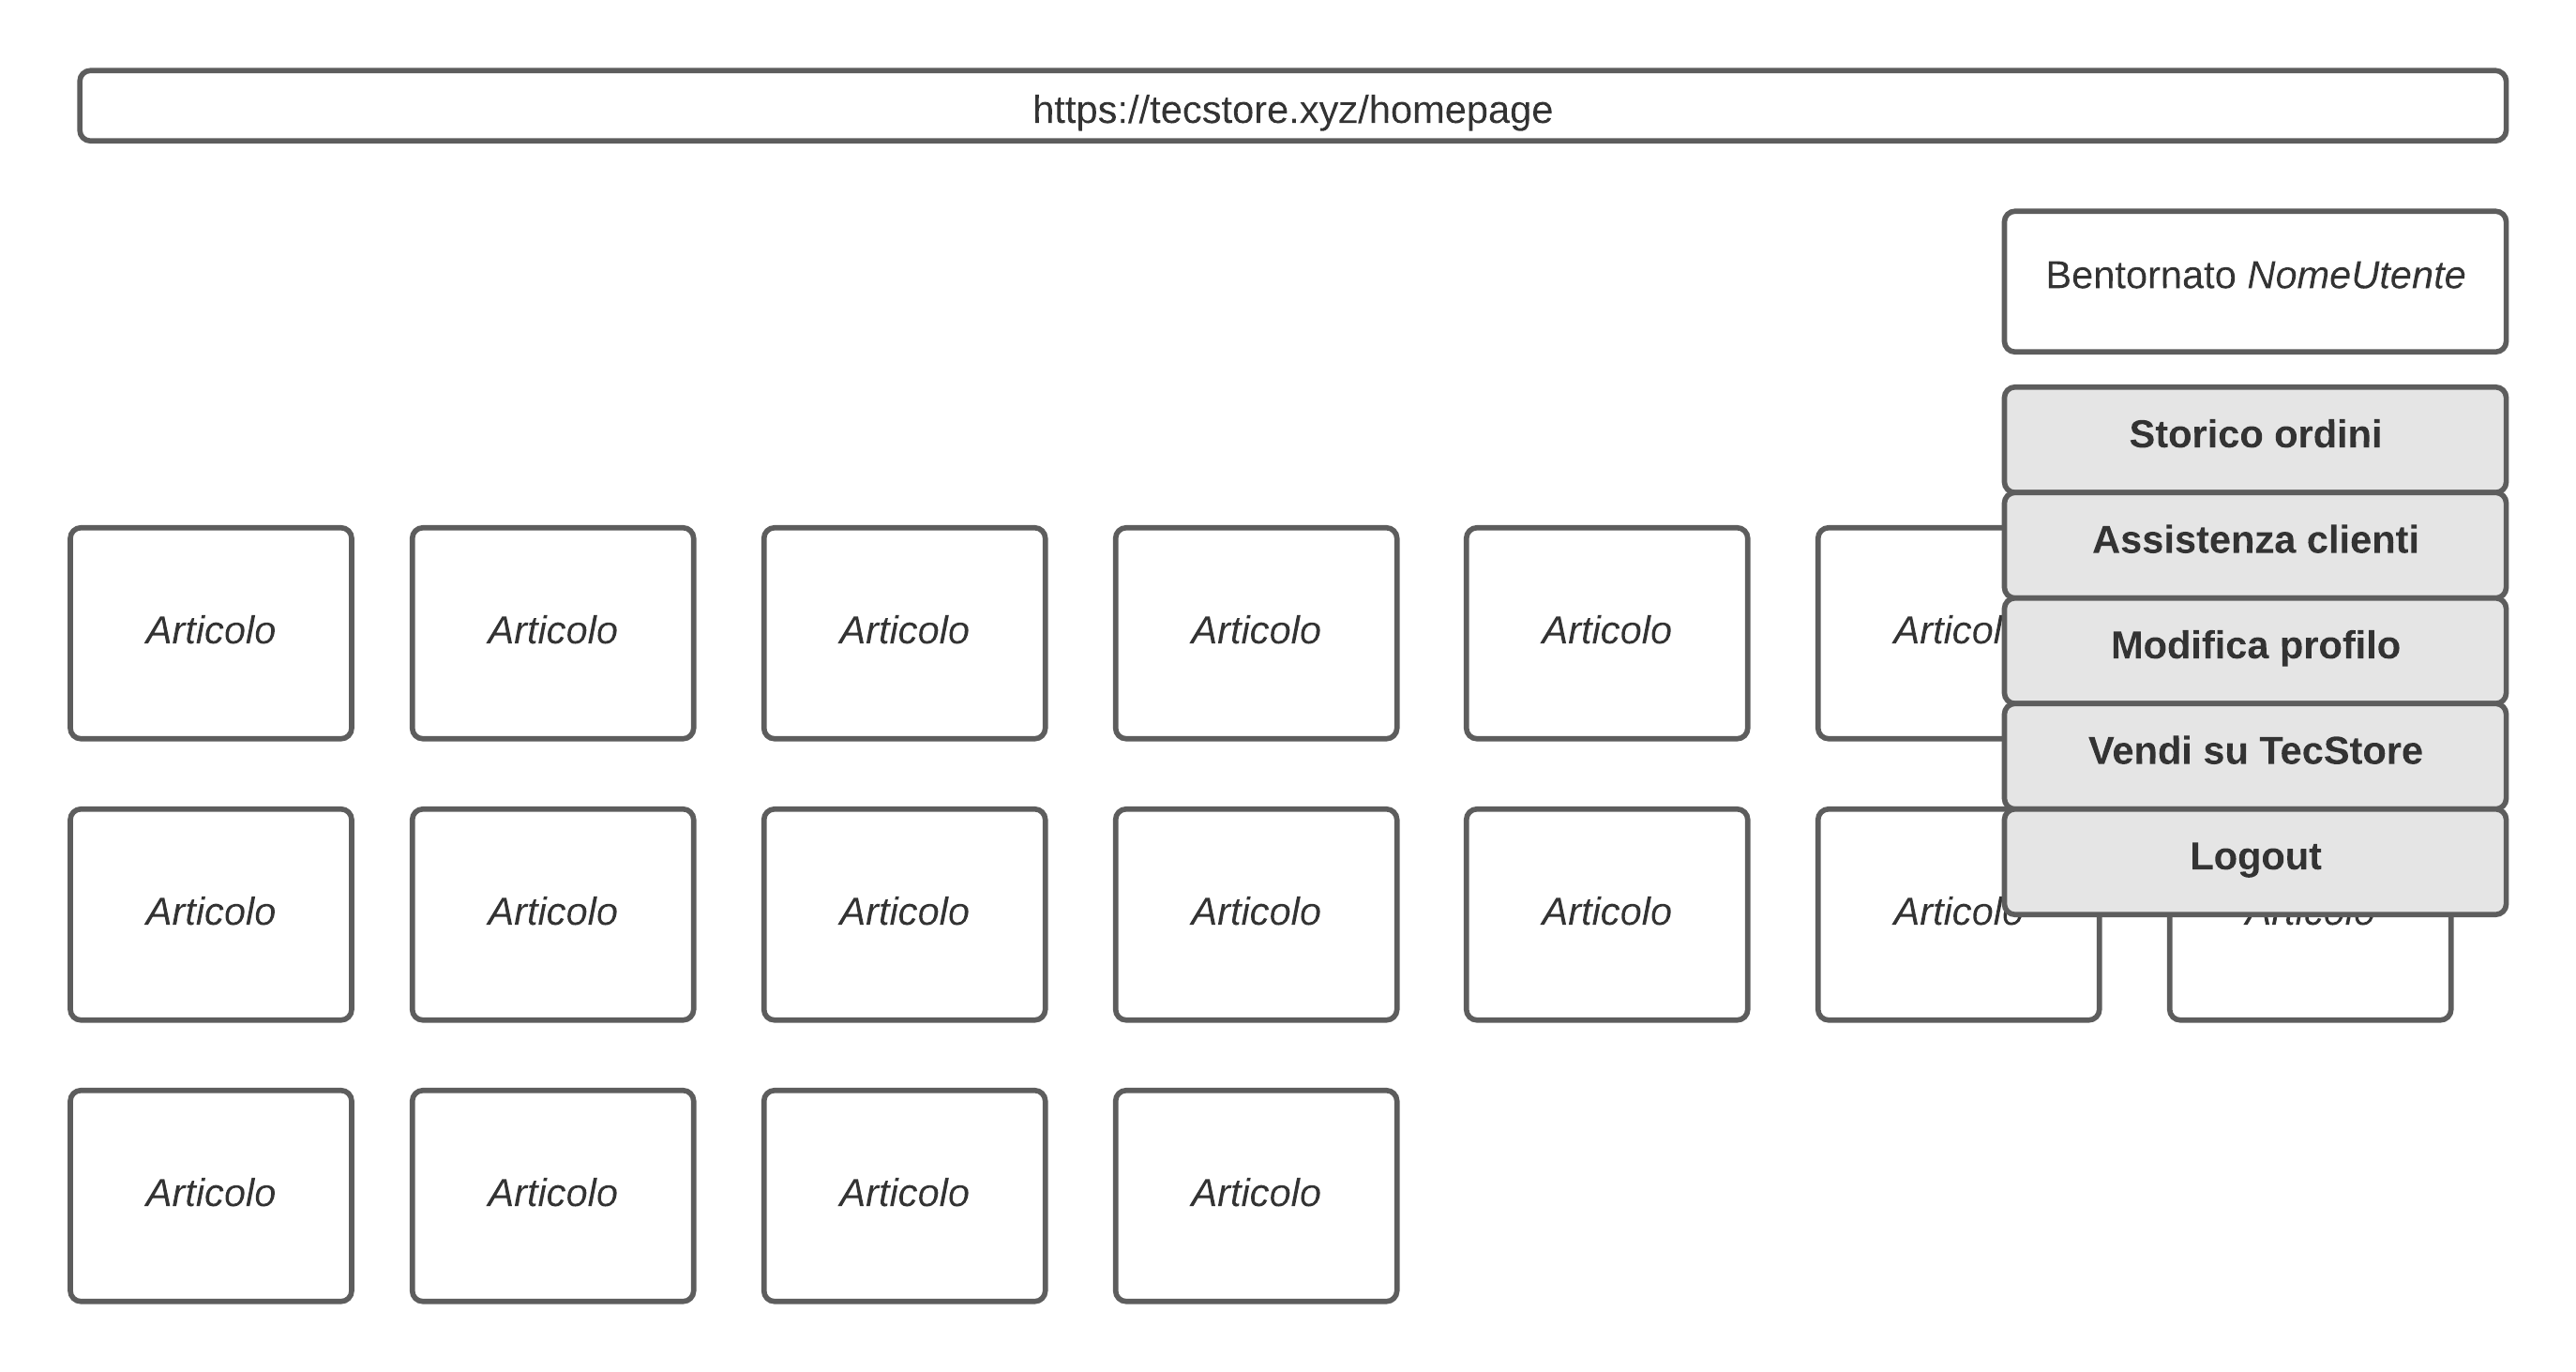
\includegraphics[width=\textwidth]{homepage_login}

\item Viene reindirizzato ad una pagina contenente il form per i dati dell'articolo e inserisce, in ordine, "Monitor AOC 22B2H", "Monitor 21.5'' 1080p 75Hz, VGA, HDMI Nero", "8" e "122.25€ e carica alcune foto del dispositivo.

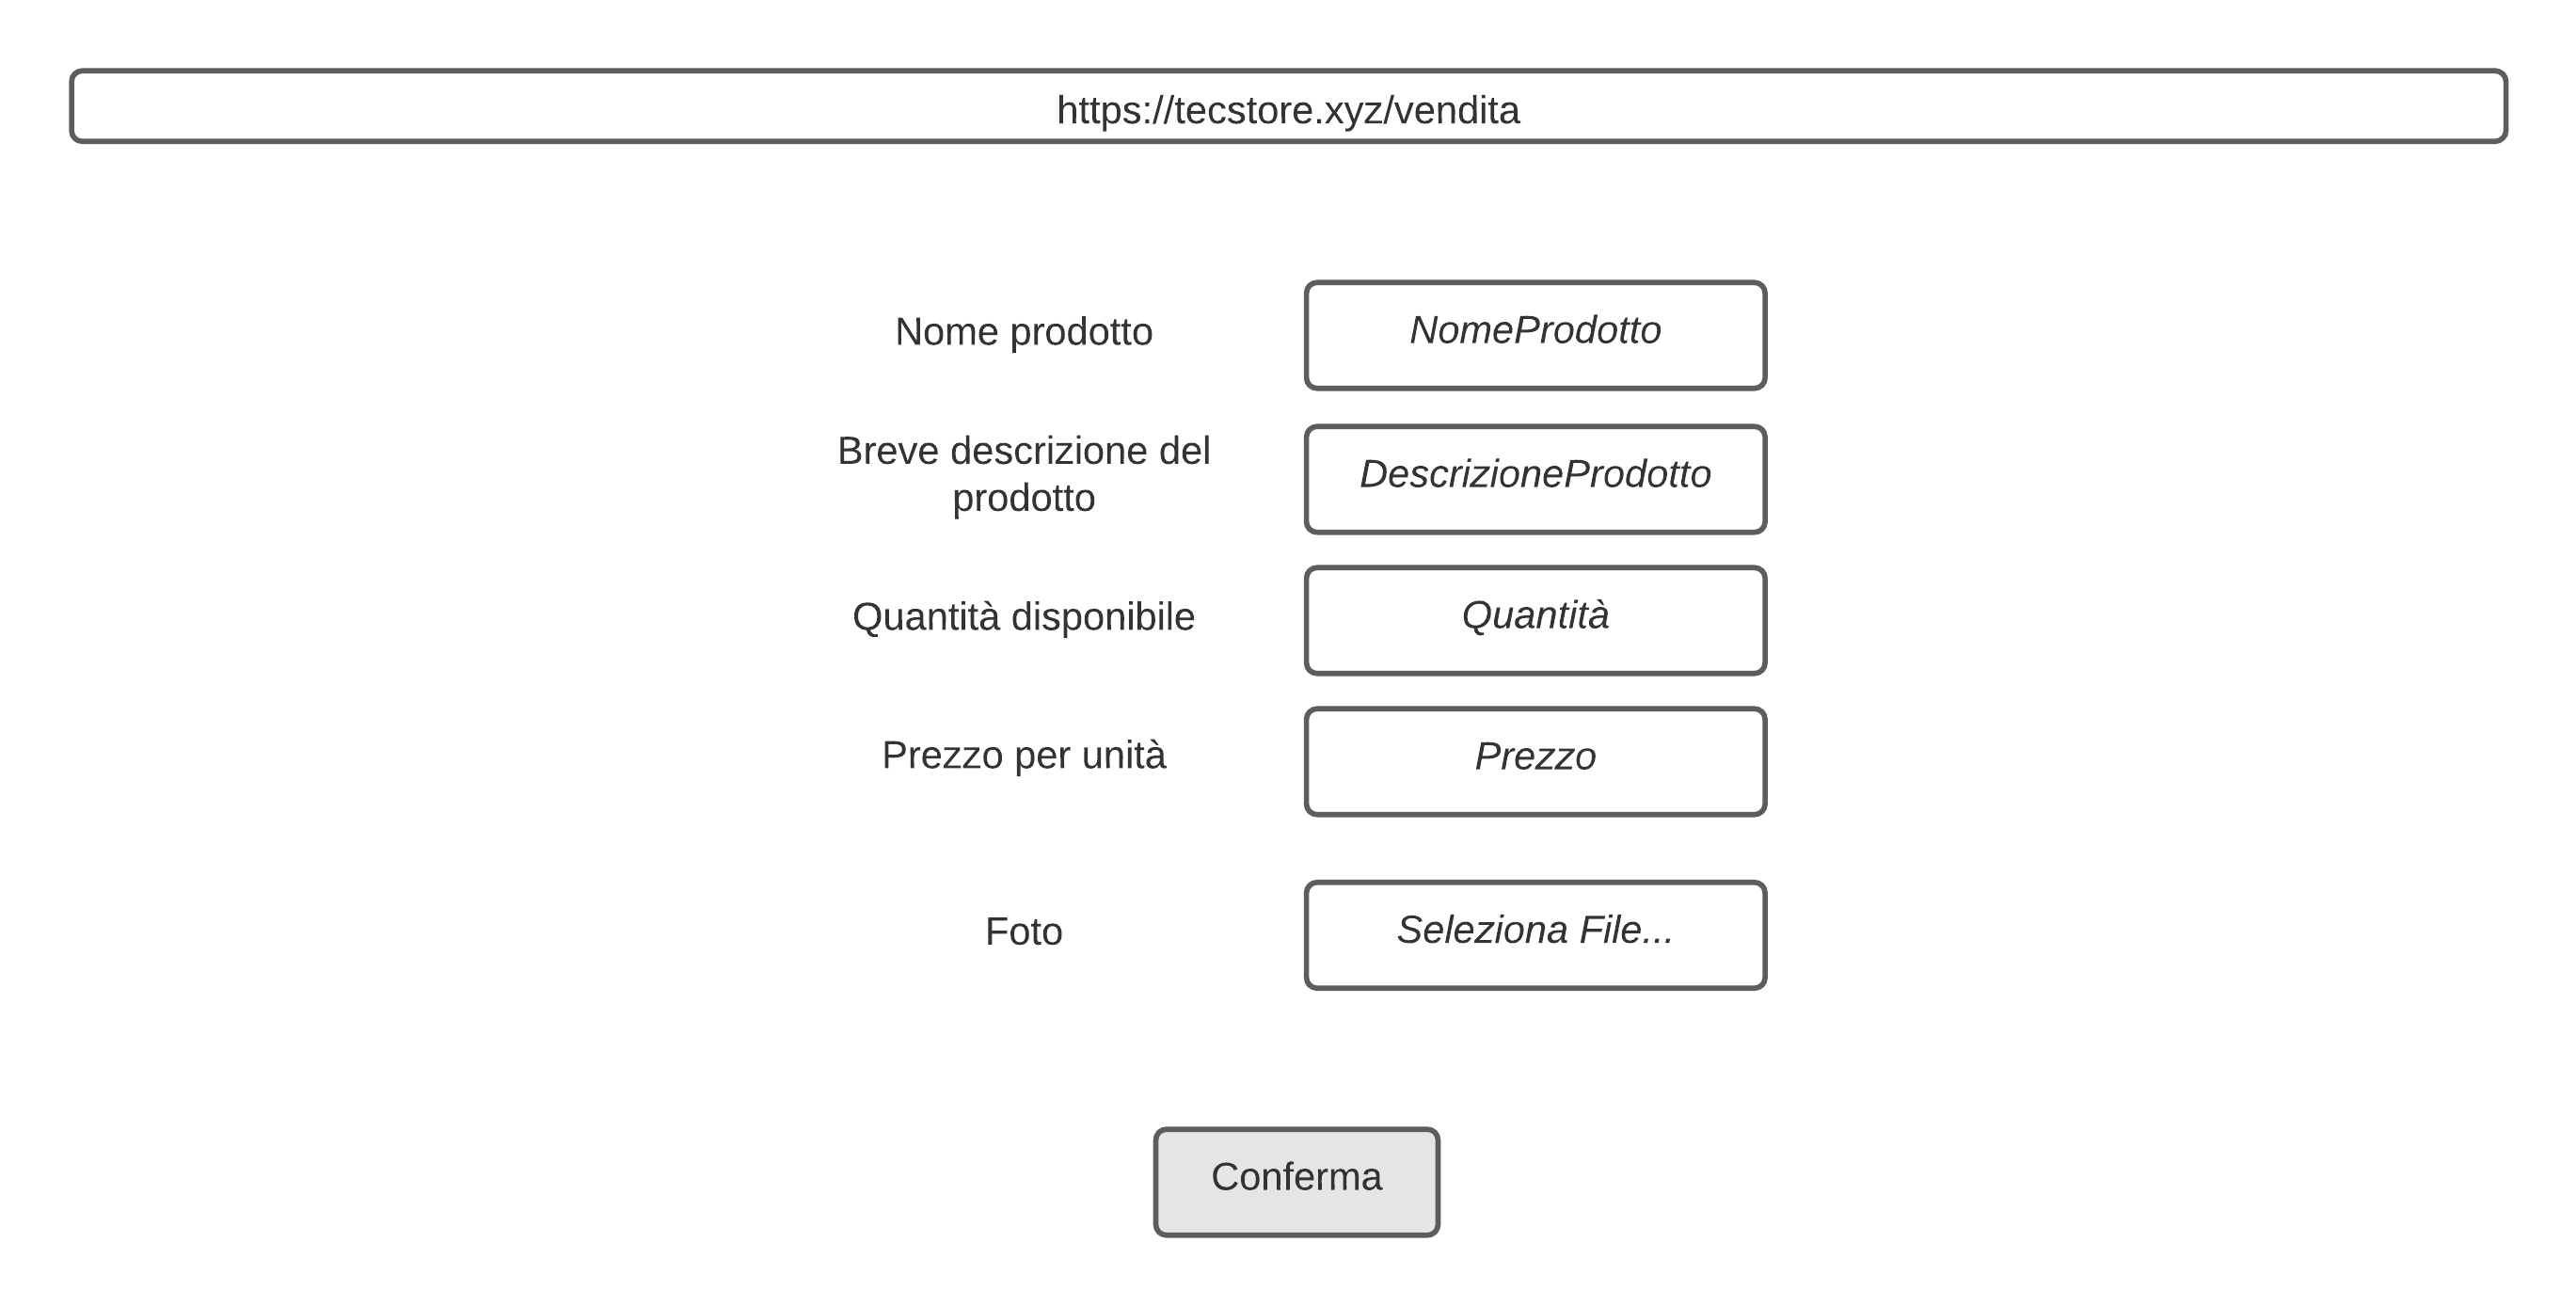
\includegraphics[width=\textwidth]{vendita}

\newpage
\item Pochi istanti dopo, un sistema automatico effettua un controllo sommario sul contenuto dell'inserzione e, dato che non contiene profanità o altri contenuti indesiderati, Silvana riceve una notifica nella sua \textit{dashboard}, richiedendo una conferma manuale all'inserimento dell'ordine nel catalogo.

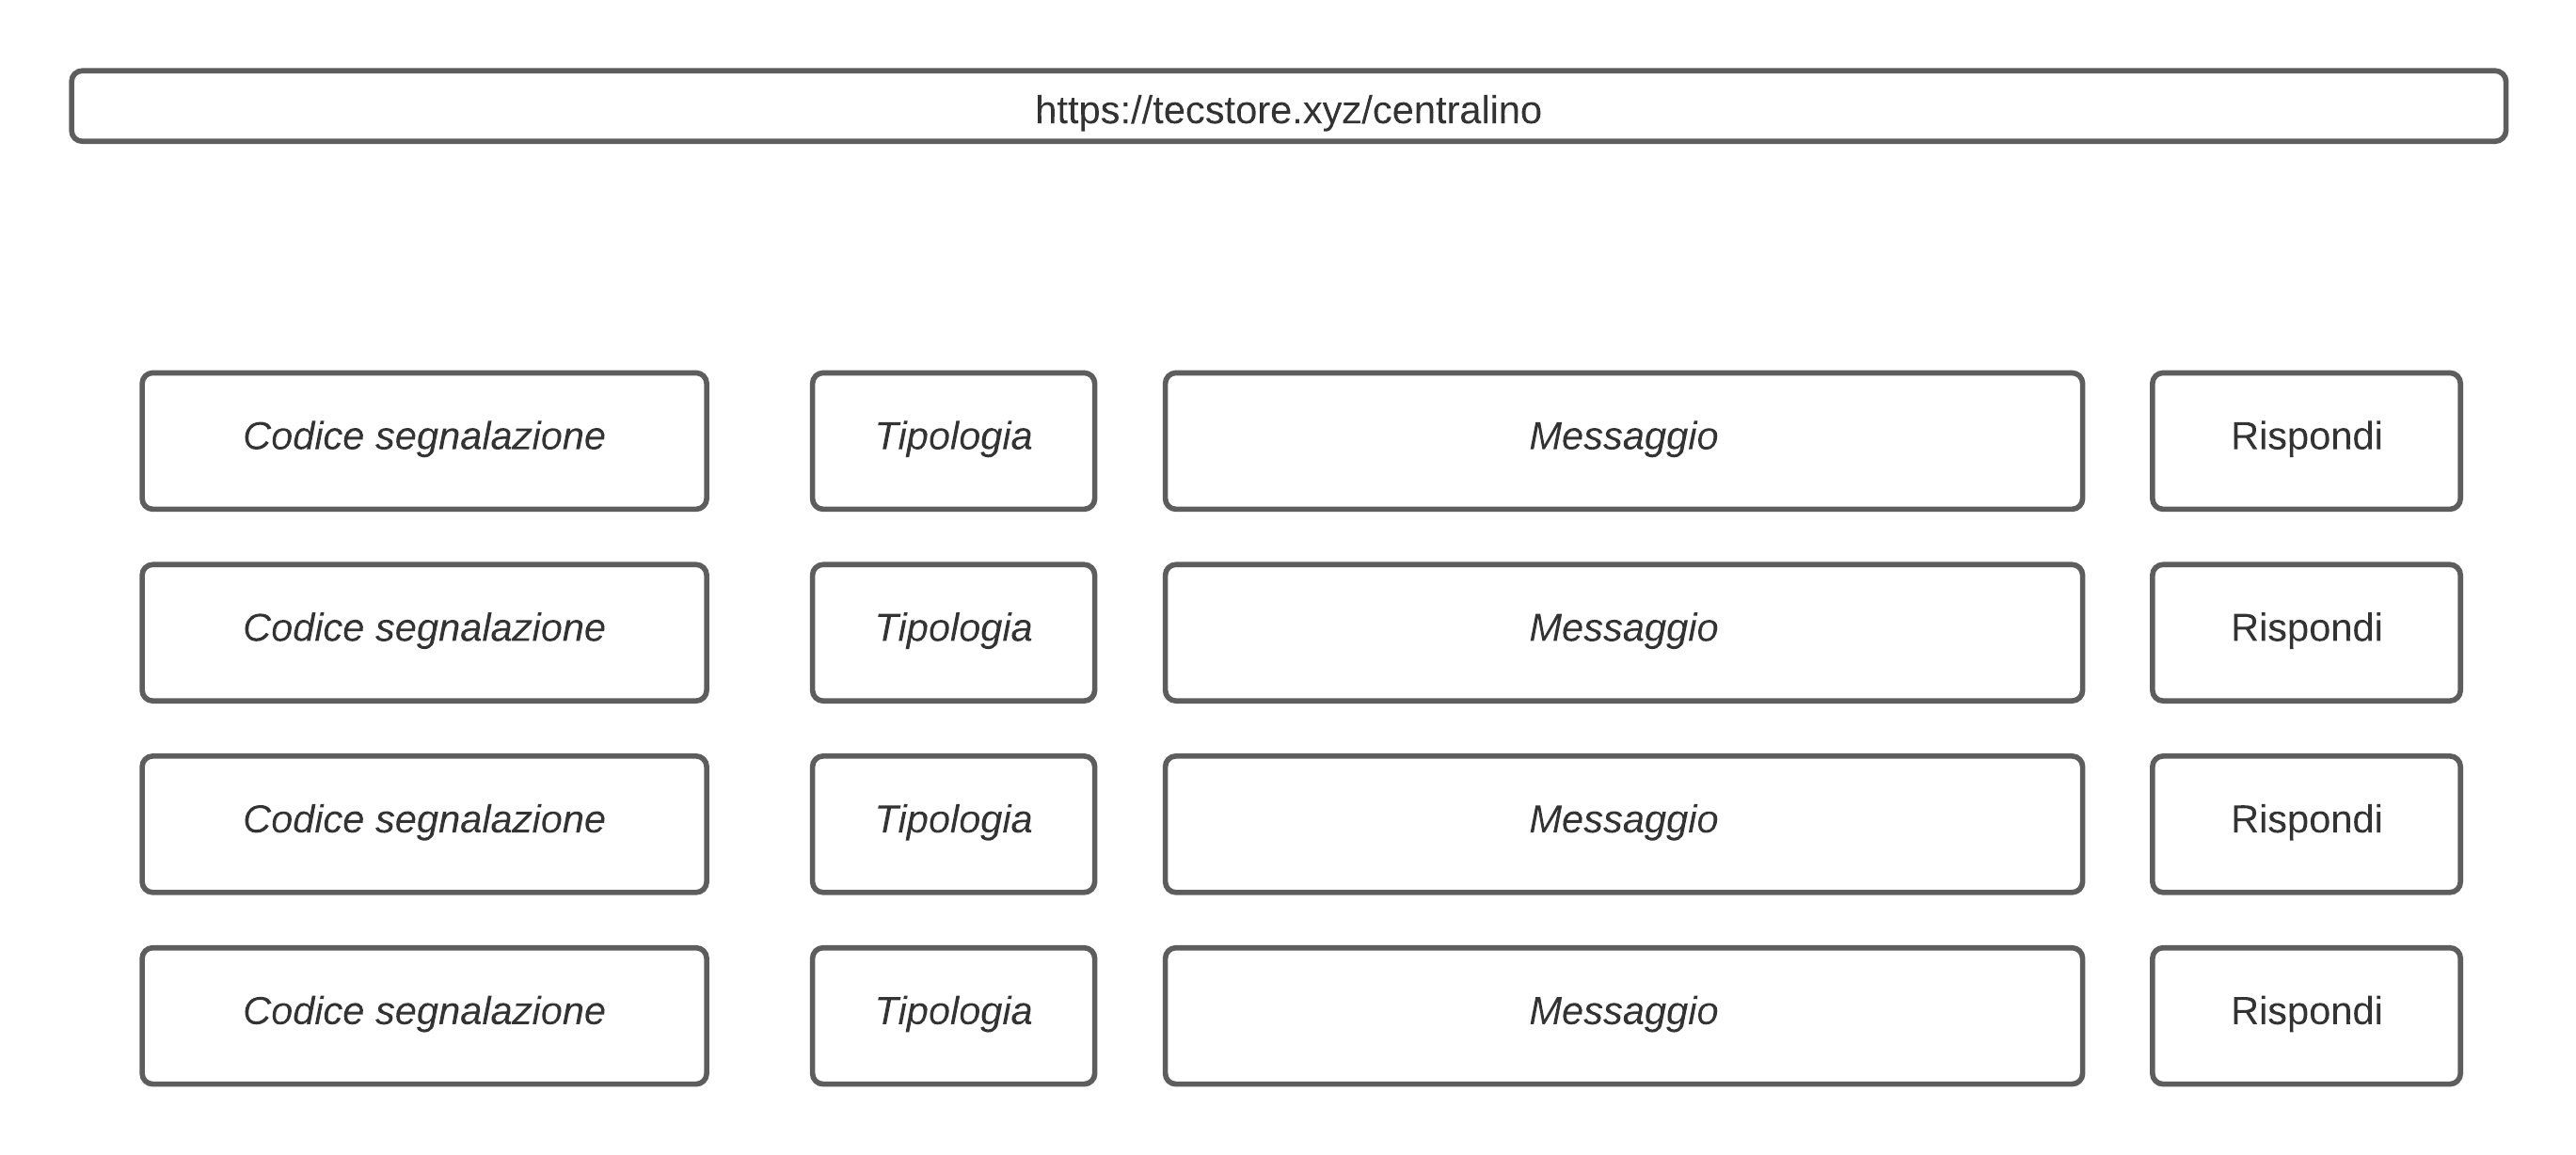
\includegraphics[width=\textwidth]{centralino}

\item Dopo aver effettuato delle ulteriori verifiche, Silvana decide di accettare l'inserzione di Alfonso, che apparirà a tutti gli altri utenti.
\end{enumerate}

\newpage

\subsection{Il responsabile del personale ha assunto un nuovo centralinista}
\textbf{Attori:} Carlo Martello, responsabile del personale e Matilde Rossi, centralinista \\

\noindent
\textbf{Flusso di eventi:}
\begin{enumerate}
\item Dopo aver sostenuto un colloquio, Matilde è stata assunta come nuova centralinista. Carlo ha il compito di registrare l'identità di Matilde nel sistema, in modo che possa lavorare.

\item Carlo effettua dalla homepage fa click sul pulsante "login" e inserisce le credenziali "HR1" e "waU9qGBrTQ3yXk21MZwo"

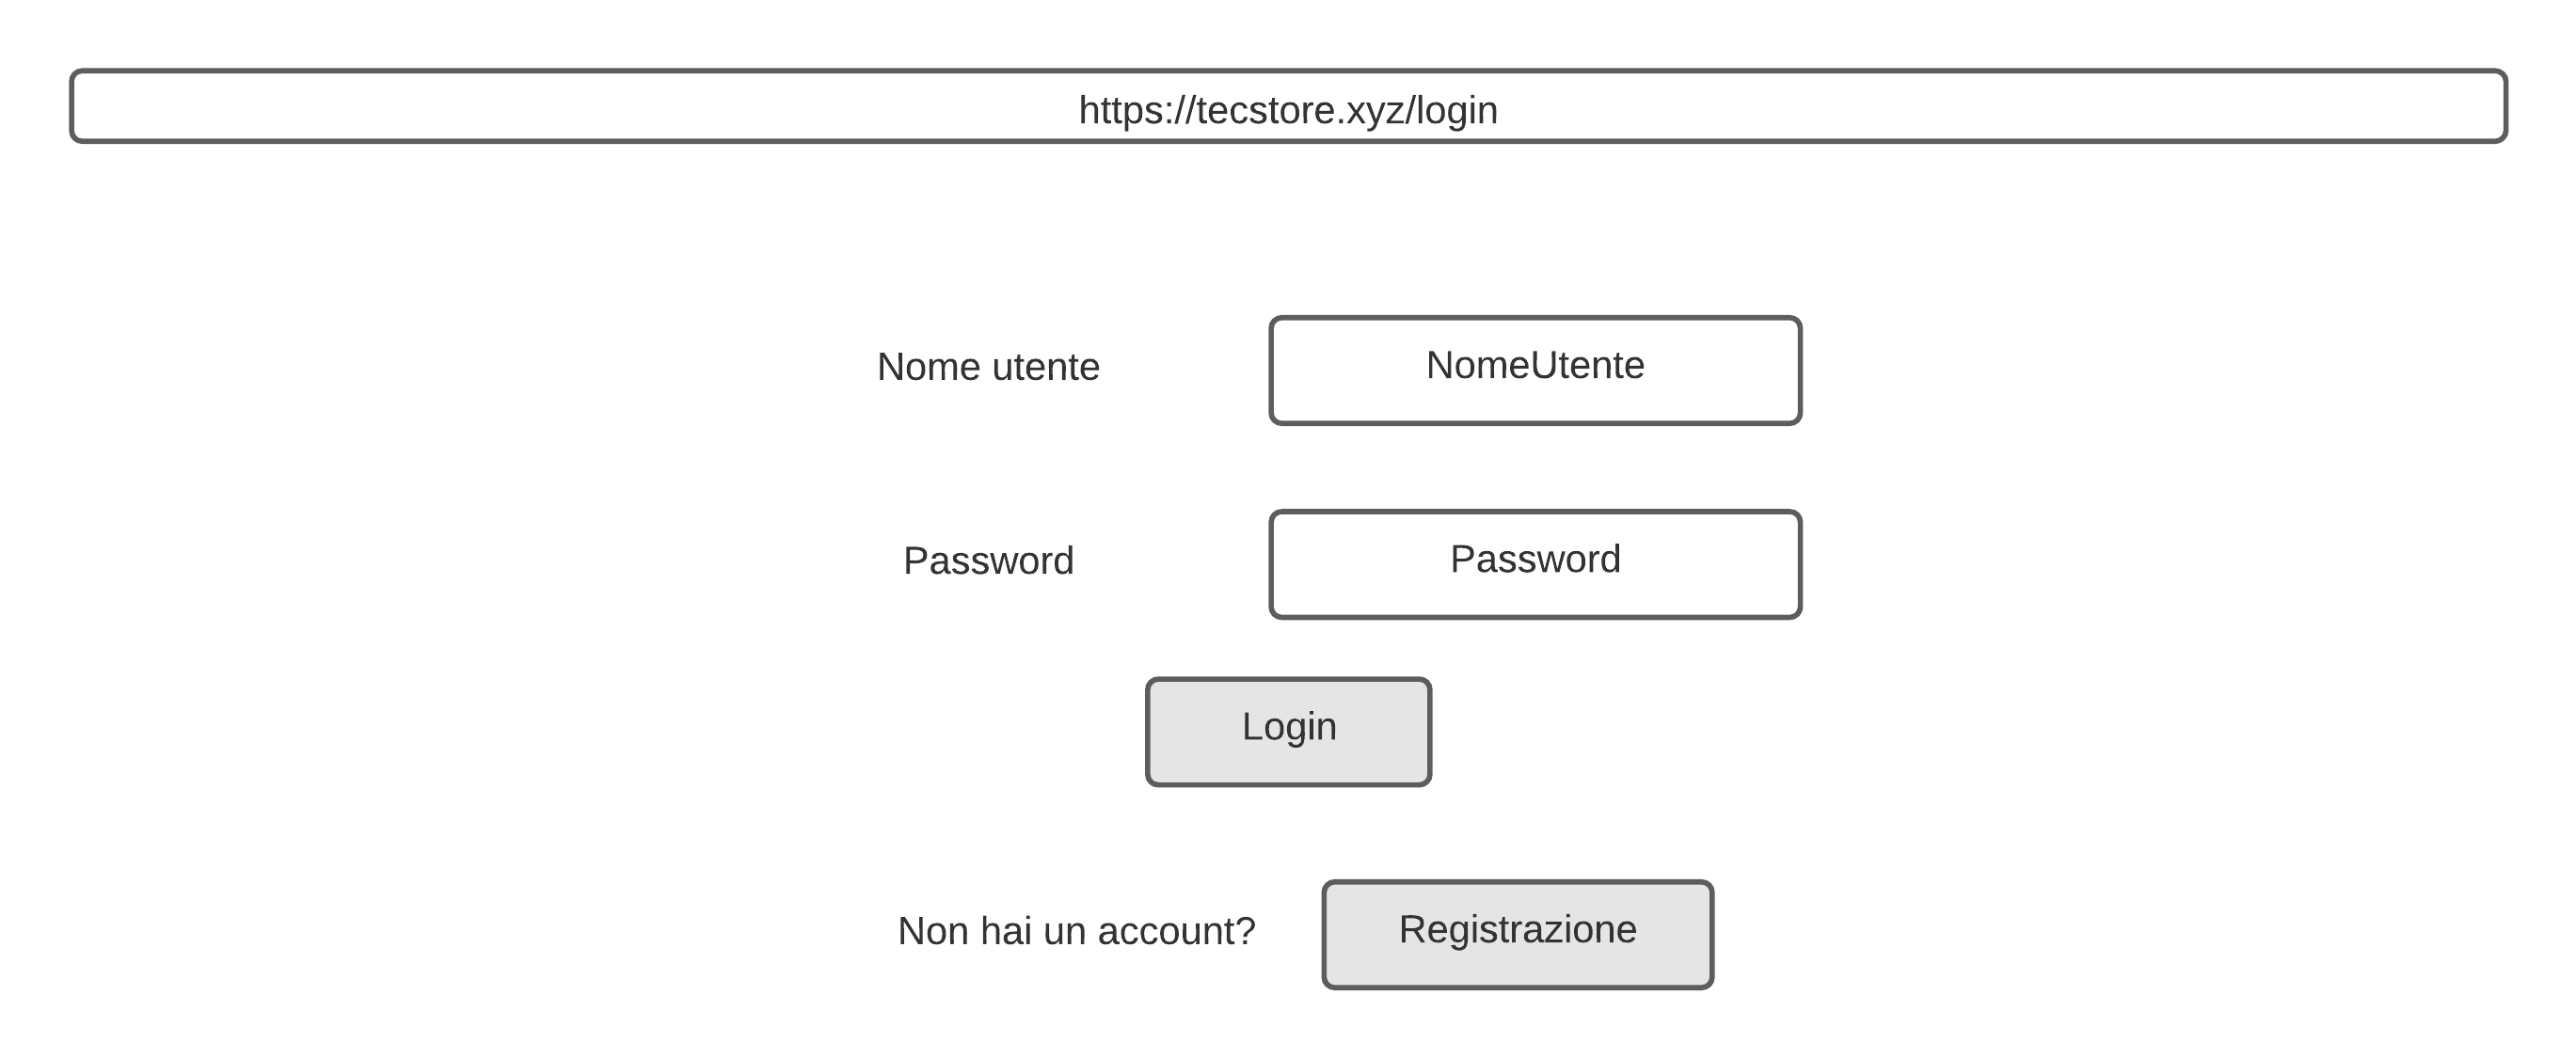
\includegraphics[width=\textwidth]{login}

\newpage
\item Viene reindirizzato alla pagina per la gestione del personale, dalla quale fa click sul pulsante per aggiungere un nuovo dipendente

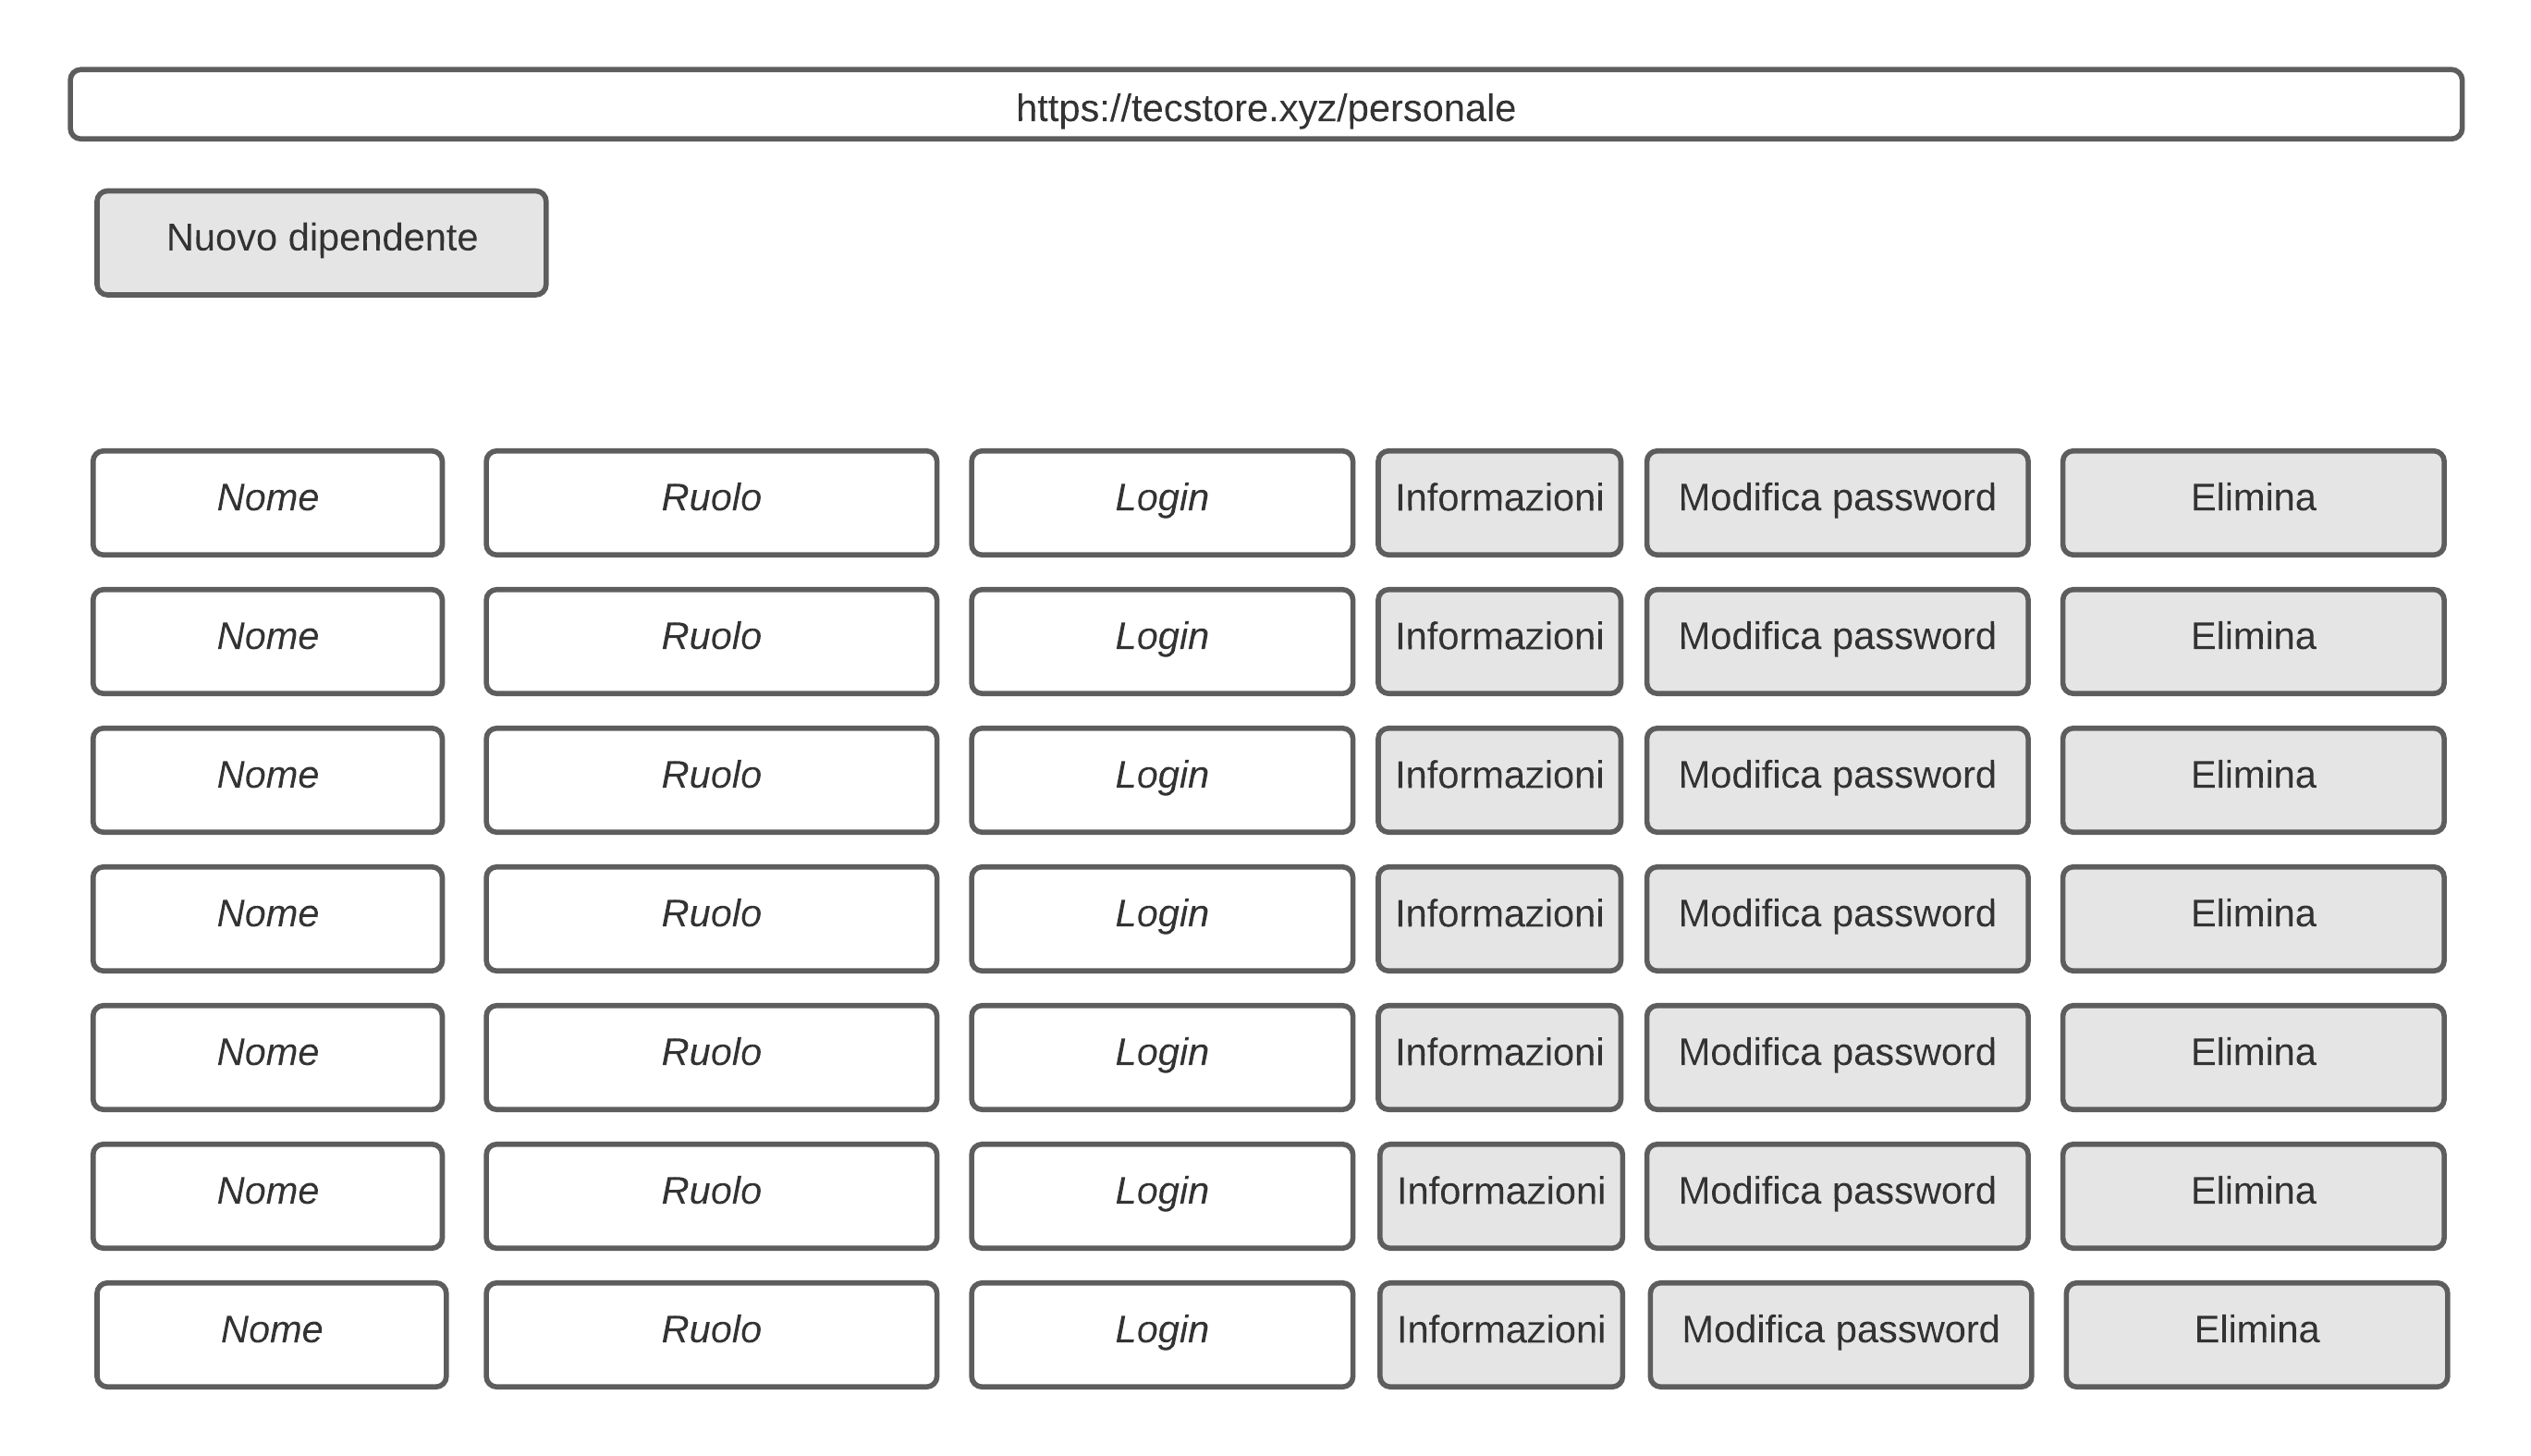
\includegraphics[width=\textwidth]{personale}

\item Viene reindirizzato al form per la creazione di un nuovo dipendente, in cui inserisce, in ordine, "Matilde", "Rossi", "21/04/1987", "Roma", "RSSMLD87D61H501M", "Roma", "Via Torino, 1", "IT18T0300203280984179265554", "Centralino" e fa click su conferma.

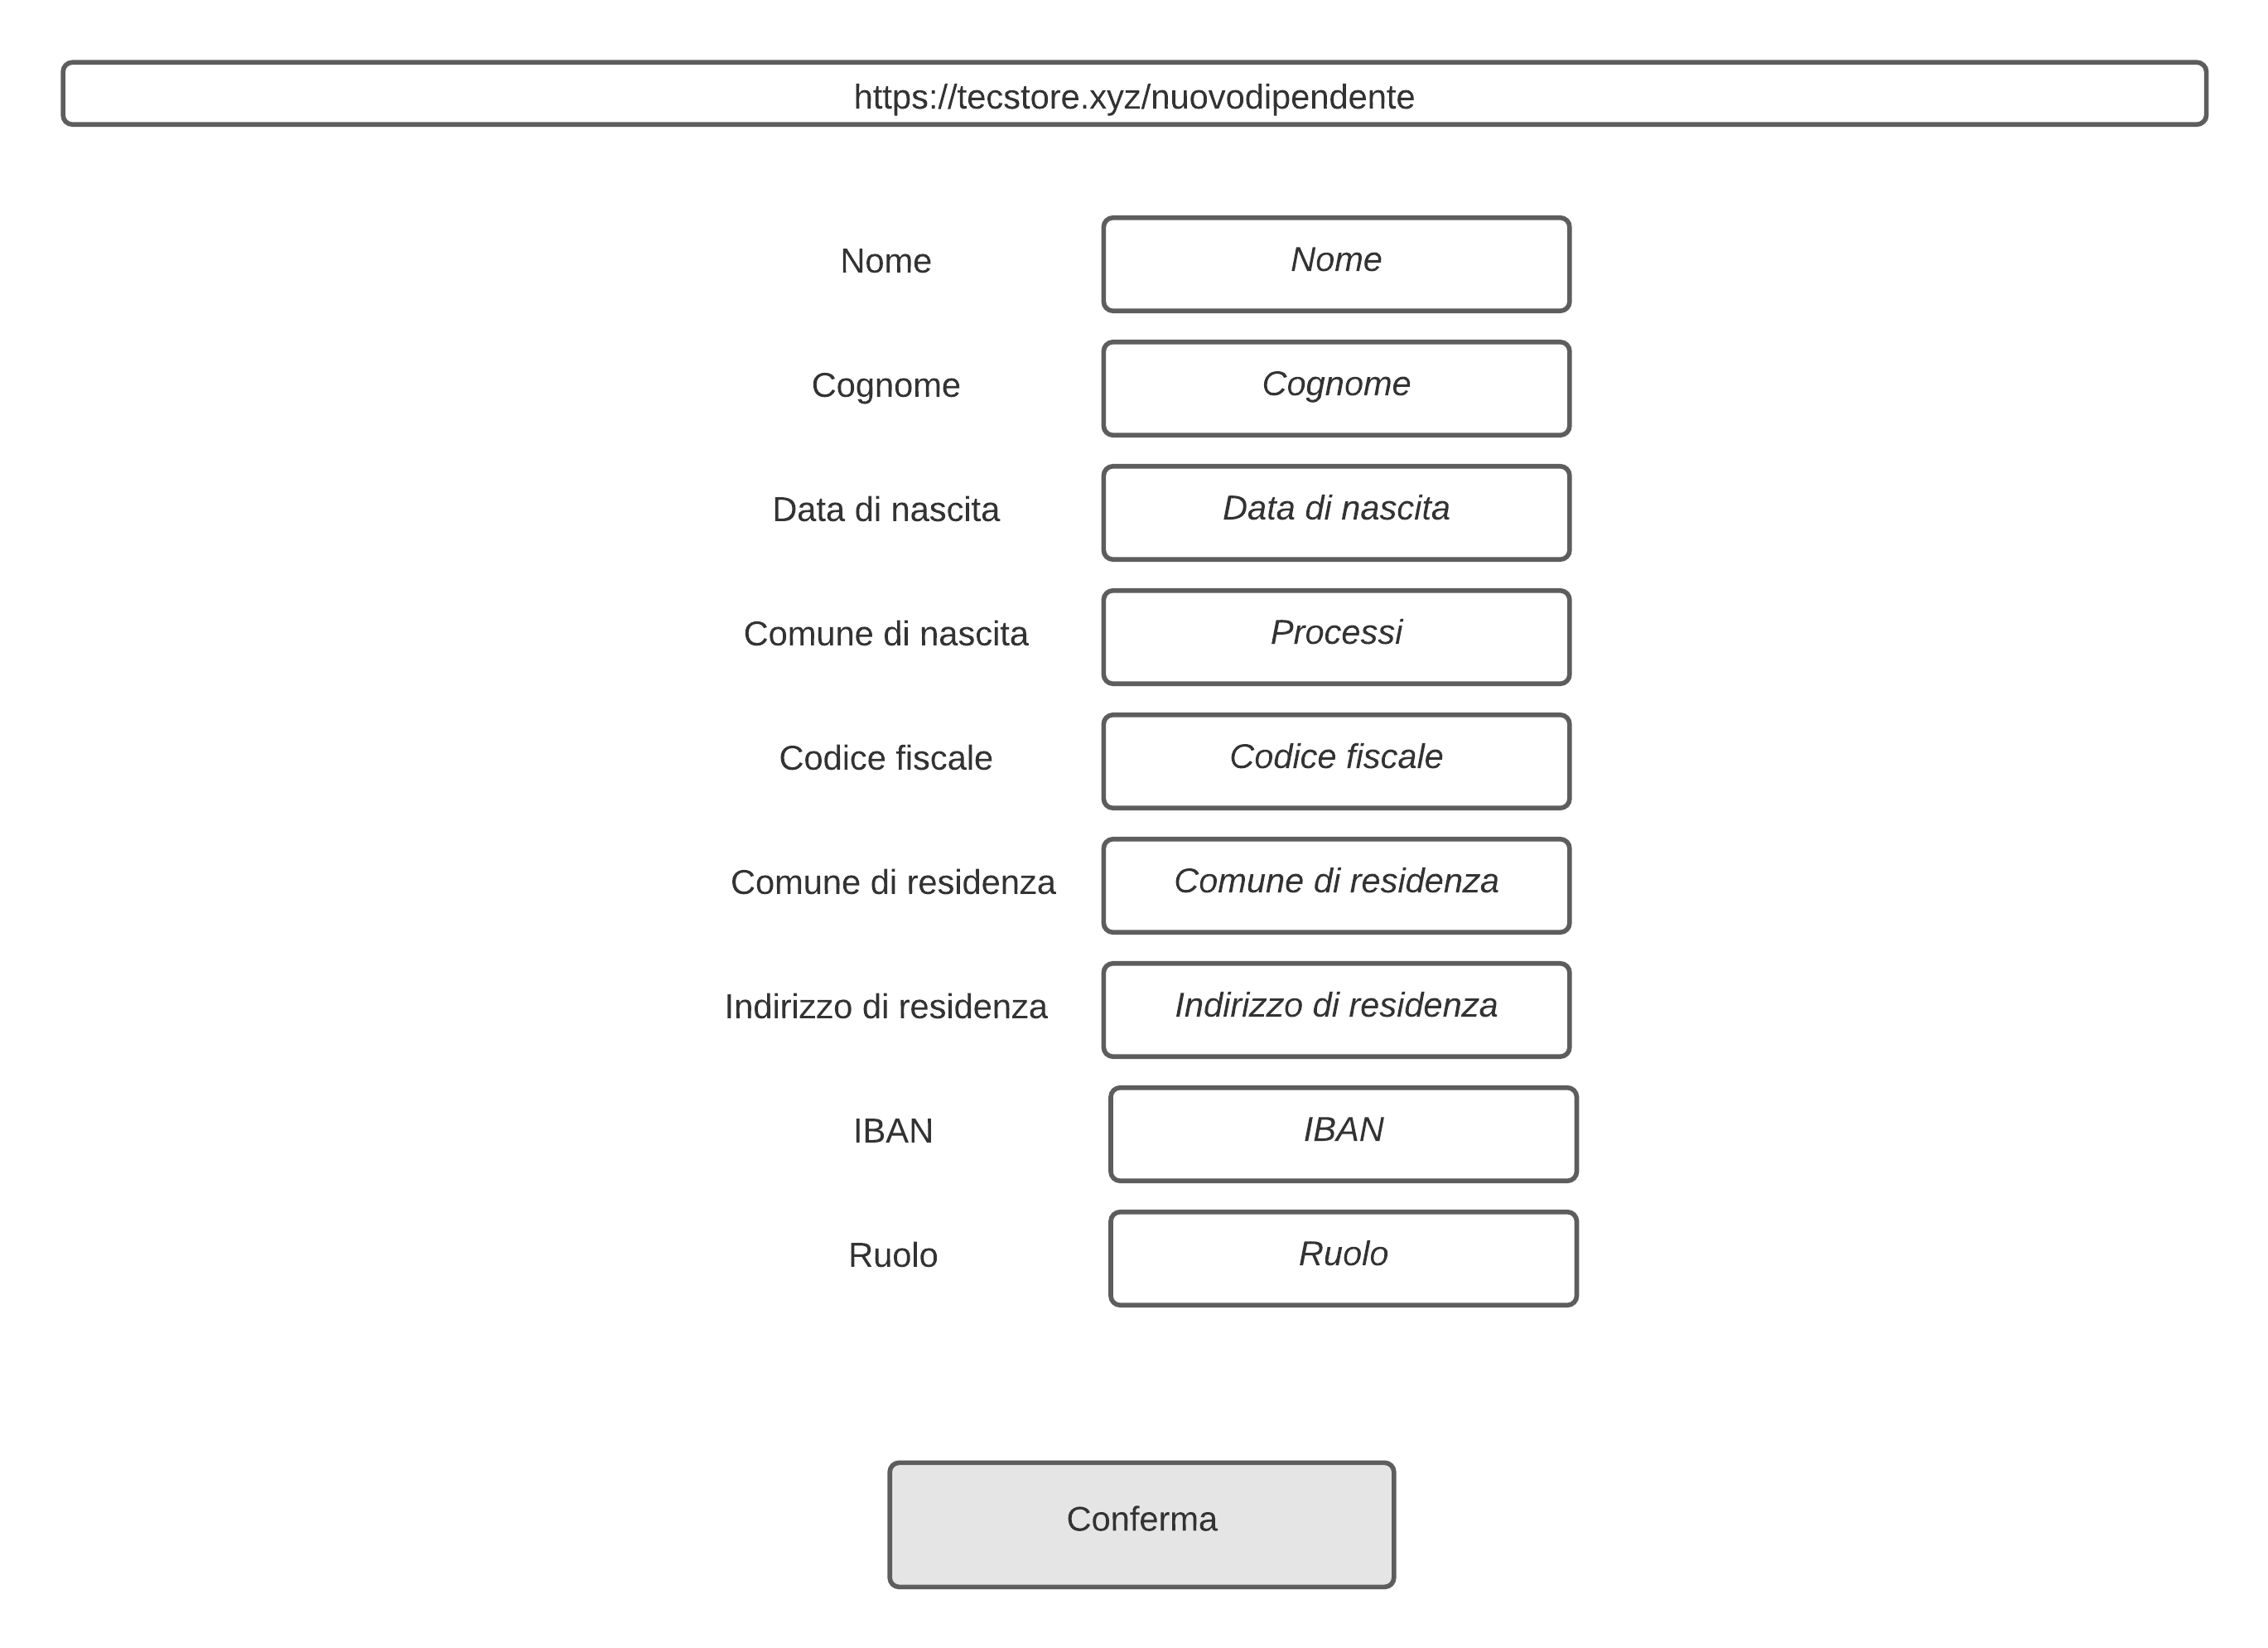
\includegraphics[height=210px]{nuovodipendente}

\item Viene mostrata una pagina contenente le informazioni di accesso per Matilde generate dal sistema, con un avviso di stampare i dati e conservarli in un luogo sicuro.

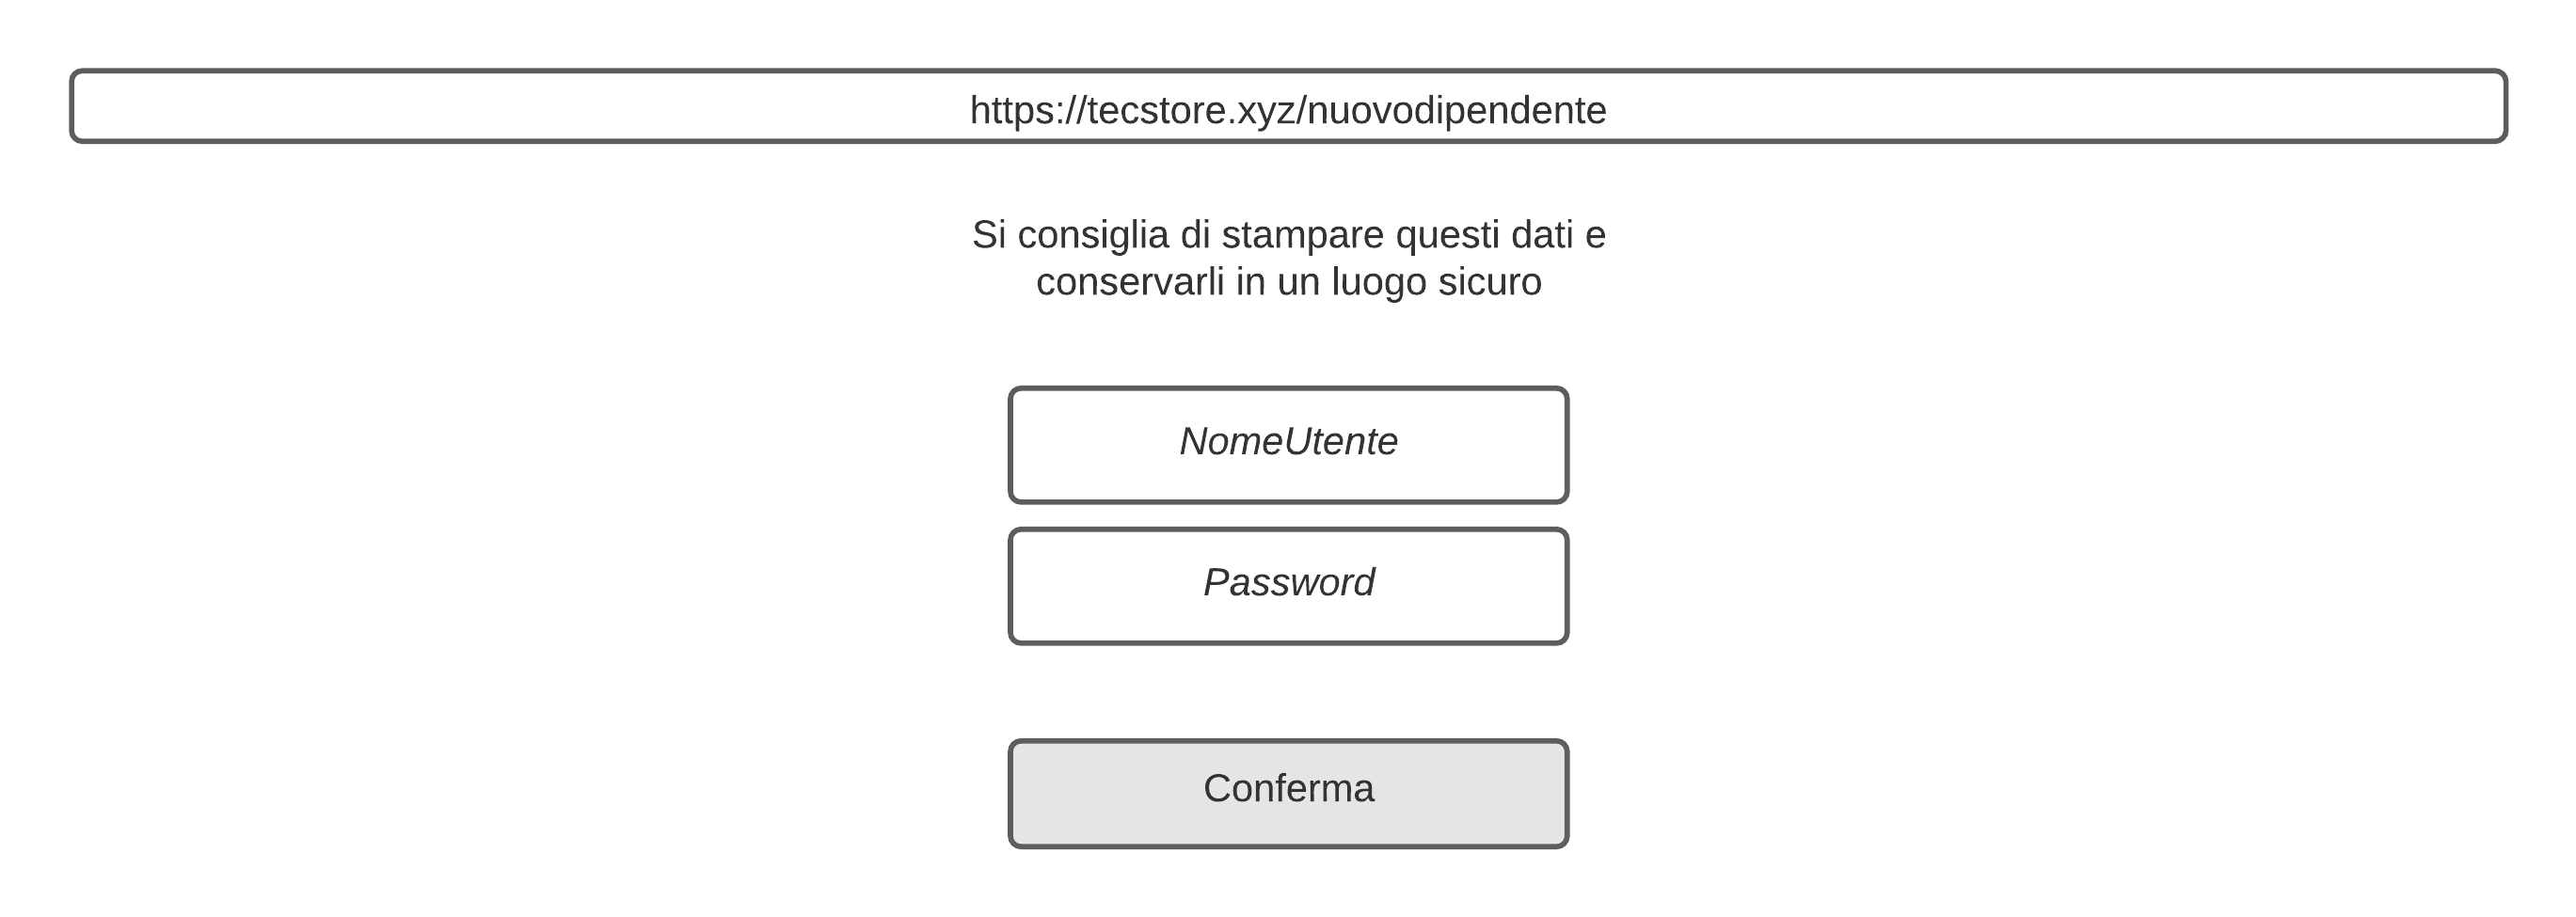
\includegraphics[width=\textwidth]{nuovodipendente2}

\item Il lunedì successivo Matilde inizia il suo primo giorno di lavoro e utilizza le credenziali ricevute per accedere alla pagina del centralino.

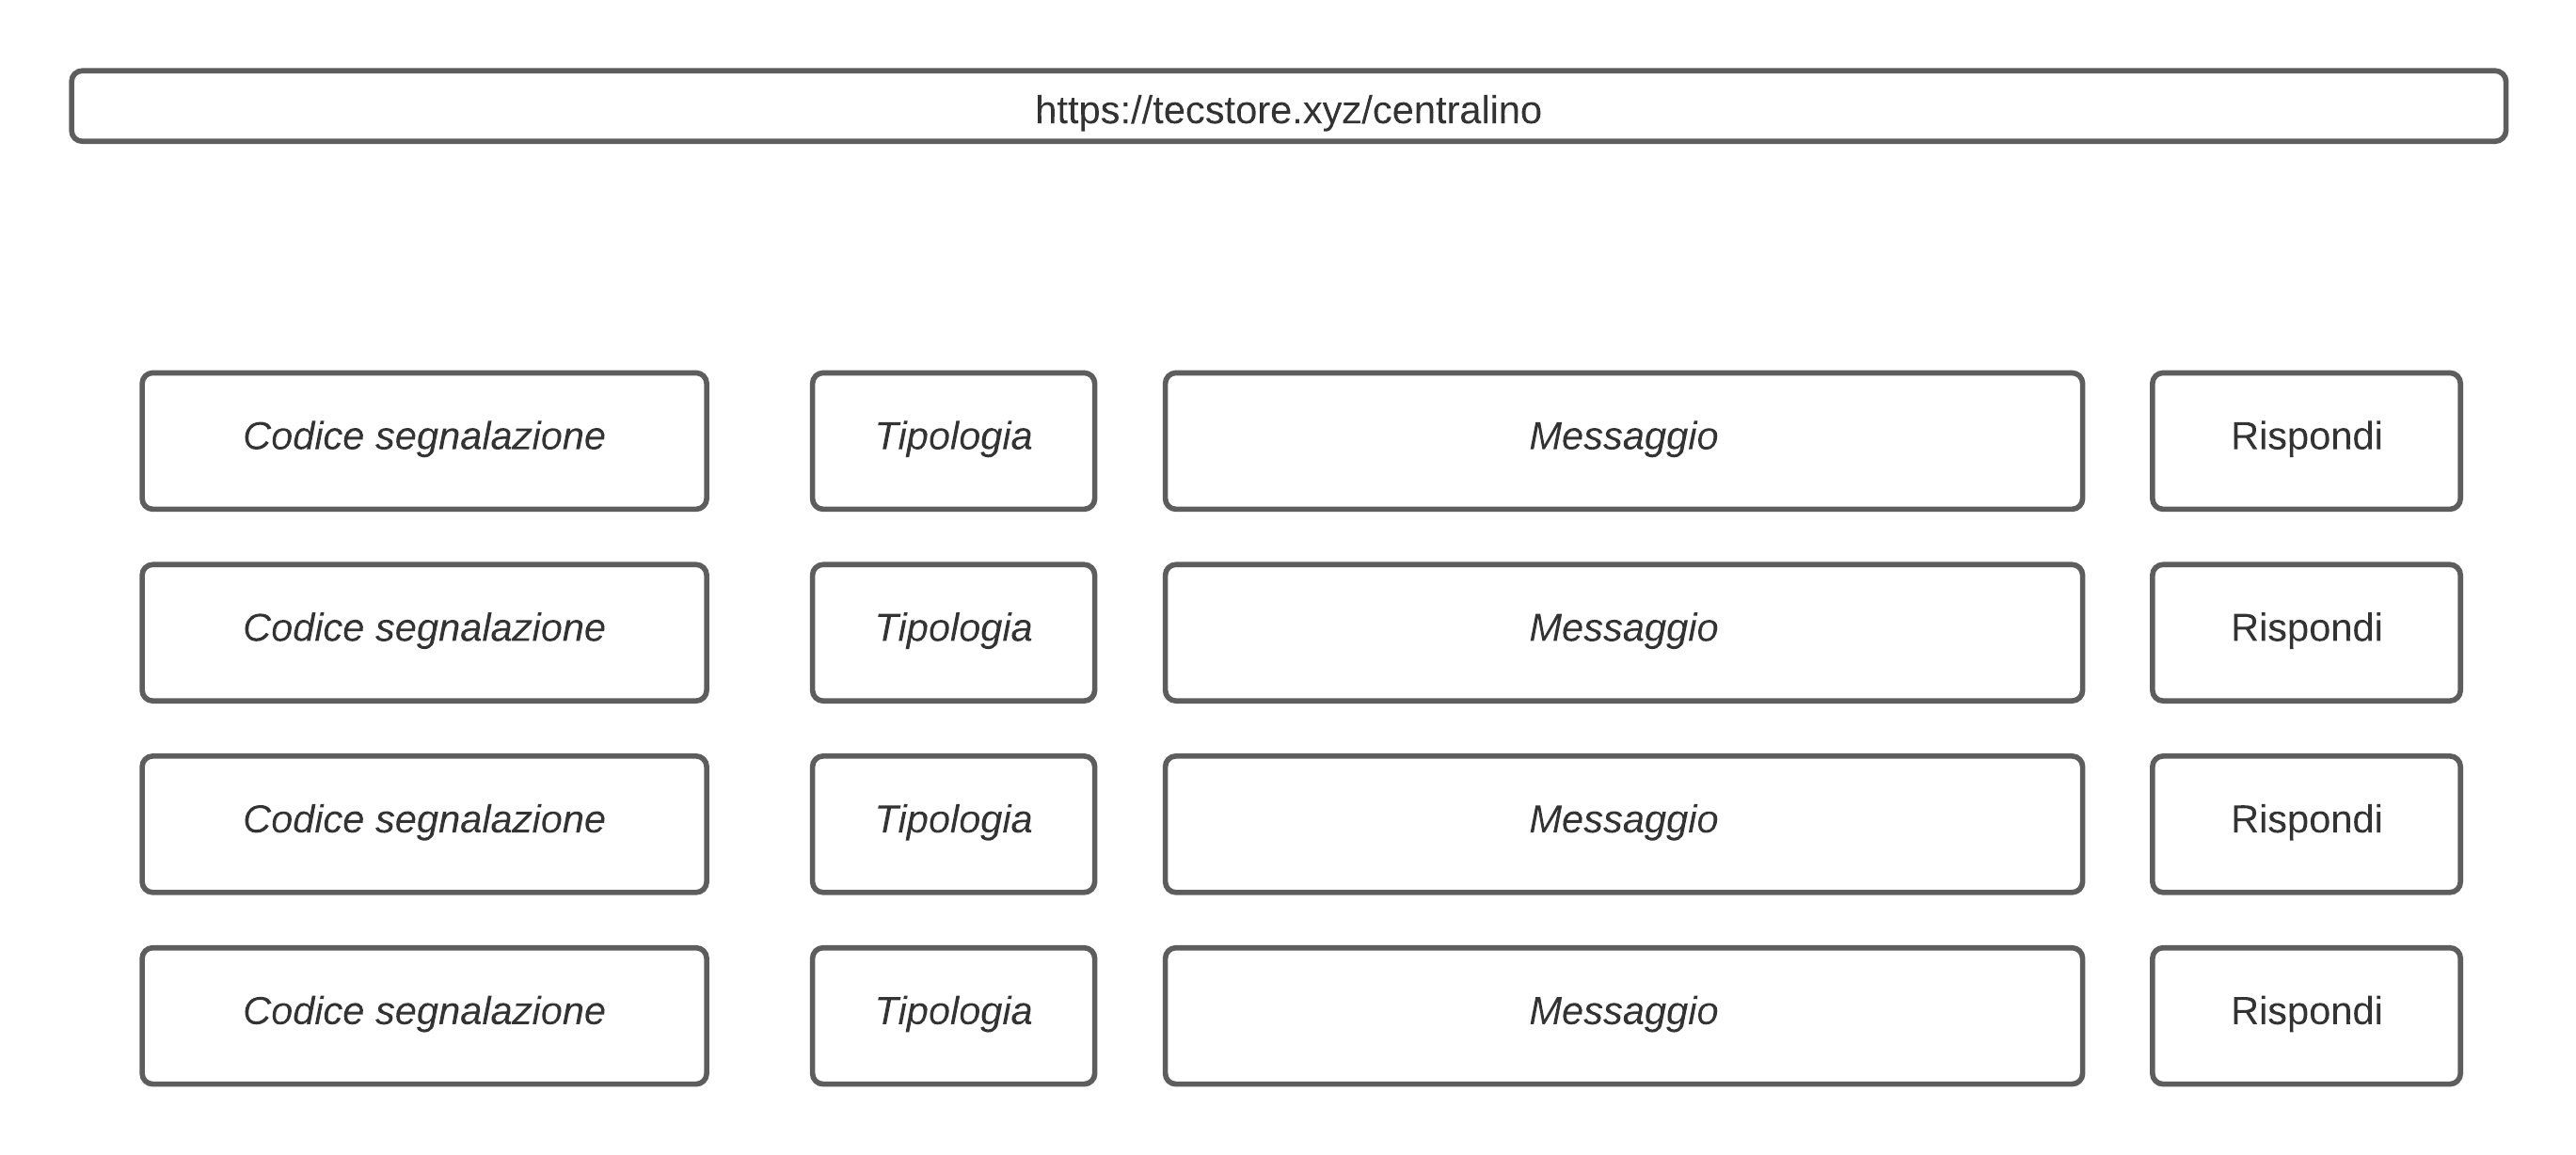
\includegraphics[width=\textwidth]{centralino}

\end{enumerate}

\newpage
\section{Requisiti funzionali}
\subsection{Clienti}
\subsubsection{Registrazione}
Il sistema deve permettere la registrazione a qualsiasi utente che lo desideri, mantenendo l'univocità dell'indirizzo email e assicurandosi che ogni password rispetti dei requisiti minimi di sicurezza come una lunghezza minima di 12 caratteri e l'utilizzo di più caratteri alfanumerici.

\subsubsection{Autenticazione}
Ad un utente registrato deve essere fornita la possibilità di effettuare il login con l'indirizzo email e la password scelti durante la registrazione. In caso di smarrimento della password, all'utente deve essere fornita la possibilità di cambiarla, ma non di recuperare la password attualmente impostata per motivi di  \hyperref[sec:security]{sicurezza}. All'utente deve essere fornita anche la possibilità di cambiarla in qualsiasi momento, ma non deve essere possibile modificare l'indirizzo email.

\subsubsection{Possibilità di acquisto di articoli solo per utenti registrati}
Il sistema deve permettere l'acquisto di articoli e la vendita di essi solo ad utenti pienamente registrati. Un utente non registrato deve solo poter consultare il catalogo ed effettuare la registrazione.

\subsubsection{Possibilità per ogni utente di vendere articoli}
Per ogni utente registrato deve essere possibile introdurre articoli nel catalogo, se passano i controlli.

\subsubsection{Possibilità di contatto del servizio clienti}
Il sistema deve rendere possibile la comunicazione con l'assistenza clienti, per evitare che un cliente non soddisfatto dai servizi diffonda cattiva pubblicità. Ciò è gestito attraverso il meccanismo dei \textit{ticket}.

\subsubsection{Modifica informazioni profilo}
All'utente deve essere permesso di cambiare password, email, indirizzo, numero di carta di credito.

\subsubsection{Recupero password}
All'utente deve essere permesso di recuperare la sua password in caso di smarrimento, anche se non è correntemente autenticato.

\subsection{Gestione piattaforma}

\subsubsection{Gestione ordini}
Il sistema deve essere provvisto di almeno un account dedicato ai magazzinieri, che si occupano dell'imballaggio e spedizione degli articoli ordinati. Un magazziniere deve avere la possibilità di annullare un ordine in caso di problemi di spedizione. L'interfaccia per il magazzino deve eventualmente prevedere una modalità "touch" per l'utilizzo semplificato con dispositivi mobile come tablet.

\subsubsection{Gestione ticket}
Il sistema deve essere provvisto di almeno un account dedicato ai centralinisti, che si occupano di gestire i rapporti con l'utenza, sia per la gestione dei ticket e quindi la risoluzione dei problemi, ma anche l'accettazione di nuovi articoli messi in vendita da un utente.

\subsubsection{Controllo di ogni articolo introdotto dall'utenza}
Per ogni articolo inserito nella piattaforma, un sistema automatico e un centralinista devono approvare il testo, per evitare oscenità e altri contenuti indesiderati.

\subsubsection{Gestione del personale da un account dedicato}
Il sistema deve essere provvisto di almeno un account con accesso all'interfaccia per la gestione degli account del personale e prevedere inserimento, rimozione e modifica degli stessi account.

\subsubsection{Gestione del catalogo da un account dedicato}
Il sistema deve essere provvisto di almeno un account con accesso all'interfaccia per la gestione del catalogo e permettere l'inserimento, rimozione e modifica di articoli nel catalogo stesso.

\section{Requisiti non funzionali}
\subsection{Sicurezza e privacy}
\label{sec:security}
Il sistema deve prevedere tutte le pratiche di sicurezza fondamentali, come l'utilizzo di SSL per la trasmissione dei dati, l'utilizzo di \textit{hashing} e \textit{salt} per le password memorizzate nel database, tutti i dati delle carte di credito e anagrafiche devono essere cifrate prima di essere inserite nel database utilizzando una cifratura robusta con una chiave che non deve essere esposta pubblicamente per nessun motivo. \\
In accordo con il Regolamento UE 2016/679, anche noto come General Data Protection Regulation, "GDPR", all'utente sarà descritto l'utilizzo che si farà dei dati raccolti durante il suo uso della piattaforma e sarà possibile la cancellazione totale di tutti i dati pertinenti, meno i dati necessari al mantenimento di un inventario accurato. \\
In caso di tentativo di accesso a schermate riservate da parte di un utente consumatore o viceversa, ovvero un utente del personale che cerca di accedere al catalogo, deve essere previsto un avviso e un \textit{redirect} ad una pagina correttamente accessibile da quel tipo di utente.

% \subsection{Semplicità di uso delle interfacce}
% Per evitare tempi di addestramento del personale troppo lunghi, le schermate riservate devono essere semplici da utilizzare, con soltanto le funzioni essenziali.
% Allo stesso modo, per evitare confusione e potenziale perdita di clienti, le interfacce per il pubblico devono essere quanto più intuitive possibile.

\subsection{Affidabilità}
Il sistema deve garantire un \emph{uptime} di almeno il 99.9\%, ovvero un \textit{downtime} annualizzato di meno di 9 ore. Ciò è cruciale per far sì che l'utenza non venga scoraggiata dall'utilizzo di TecStore come negozio primario, creando perdite potenziali molto alte. \footnote{https://www.the20.com/blog/the-cost-of-it-downtime/}

\subsection{Performance}
Il sistema deve prevedere la possibilità di utilizzo di sistemi di \textit{load balancing} per distribuire il carico di utenza in caso di picchi improvvisi tra più server, in modo da garantire l'uso della piattaforma al maggior numero di clienti possibile.

\subsection{Manutenibilità}
Il sistema sarà progettato secondo principi di sviluppo che ne garantiranno la semplicità di aggiornamento, ampliamento e modifica.
Sarà utilizzata un'architettura Three-Tier per separare la gestione dei dati, il programma server e l'interfaccia utente.

\subsection{Implementazione}
Sarà utilizzata la tecnologia JSP con servlet su server Tomcat per la presentazione delle pagine web all'utente , un database MariaDB per la memorizzazione dei dati e ogni utente utilizzerà un comune browser web per accedere al sistema.

\section{Ambiente di destinazione}

Trattandosi di un'applicazione orientata all'utilizzo tramite Internet, il sistema sarà accessibile da qualsiasi dispositivo munito di un browser e una connessione Internet attiva, inclusi Personal Computer e smartphone.

\section{Consegne e scadenze}

\begin{center}
\begin{tabular} {| c | c |}
\hline
\textbf{Documento} & \textbf{Consegne} \\
\hline
Problem Statement & 1 dicembre 2021 \\
Requirements Analysis Document & 10 dicembre 2021 \\
System Design Document & 5 gennaio 2022 \\
Implementazione e testing & 27 gennaio 2022 \\
\hline
\end{tabular}
\end{center}
\end{document}
